% =============================================================================
% main.tex — Root document for the bachelor thesis
% =============================================================================
\documentclass[12pt,a4paper]{report}

% =============================================================================
% preamble.tex — Package imports and custom commands
% =============================================================================

% --- Page layout ---
\usepackage[left=3.5cm, right=2.5cm, top=2.5cm, bottom=2.5cm]{geometry}

% --- Line spacing ---
\usepackage{setspace}

% --- Encoding and fonts ---
\usepackage[utf8]{inputenc}
\usepackage[T1]{fontenc}
\usepackage{lmodern}
\usepackage[
  activate={true,nocompatibility},  % enable protrusion and font expansion
  tracking=true,                    % enable letter spacing adjustments
  expansion=true,                   % allow glyph scaling for better line breaks
  stretch=10,                       % max glyph stretch (per mille)
  shrink=10                         % max glyph shrink  (per mille)
]{microtype}

% --- Language ---
\usepackage[main=english,czech]{babel}

% --- PDF inclusion (SIS title pages) ---
\usepackage{pdfpages}

% --- Mathematics ---
\usepackage{amsmath}
\usepackage{amssymb}
\usepackage{bm}                    % bold math (e.g. \bm{\delta} for Newton correction)
\DeclareMathSizes{12}{11}{8}{6}    % text=12pt: math=11pt, script=8pt, scriptscript=6pt

% --- Chemistry ---
\usepackage[version=4]{mhchem}

% --- Units ---
\usepackage{siunitx}
\sisetup{
  per-mode=symbol,
  inter-unit-product=\ensuremath{{}\cdot{}}
}

% --- Graphics and figures ---
\usepackage{graphicx}
\usepackage{float}
\usepackage[section]{placeins}   % prevents floats from spilling across section boundaries
\usepackage{tikz}
\usetikzlibrary{decorations.pathreplacing}

% --- Tables ---
\usepackage{booktabs}
\usepackage{longtable}             % for symbols / abbreviations lists spanning multiple pages

% --- Figure/table captions at 9pt per supervisor's instruction ---
\usepackage{caption}
\DeclareCaptionFont{ninept}{\fontsize{9pt}{11pt}\selectfont}
\captionsetup{font=ninept, labelfont={bf,ninept}}

% --- Cross-references and links ---
\usepackage[hypertexnames=false]{hyperref}
\hypersetup{
  colorlinks=true,
  linkcolor=blue!70!black,
  citecolor=green!50!black,
  urlcolor=blue!70!black
}

% --- Smart cross-references (cleveref must come AFTER hyperref) ---
\usepackage{cleveref}
\crefname{figure}{Figure}{Figures}
\Crefname{figure}{Figure}{Figures}
\crefname{table}{Table}{Tables}
\Crefname{table}{Table}{Tables}
\crefname{chapter}{Chapter}{Chapters}
\Crefname{chapter}{Chapter}{Chapters}
\crefname{section}{Section}{Sections}
\Crefname{section}{Section}{Sections}
\crefname{subsection}{Section}{Sections}
\Crefname{subsection}{Section}{Sections}
\crefname{subsubsection}{Section}{Sections}
\Crefname{subsubsection}{Section}{Sections}
\crefname{equation}{equation}{equations}
\Crefname{equation}{Equation}{Equations}

% --- Paragraph formatting ---
\usepackage{parskip}

% --- Page-break control ---
\widowpenalty=10000          % NEVER allow single-line widow at top of next page
\clubpenalty=10000           % NEVER allow single-line orphan at bottom of page
\displaywidowpenalty=10000   % NEVER allow widow line before a displayed equation
\predisplaypenalty=10000     % keep colon-led-in line glued to its equation (no page break)
\postdisplaypenalty=500      % mild discouragement of page break just after equation
\interlinepenalty=200        % discourage page breaks inside a paragraph
\brokenpenalty=10000         % discourage page break after a hyphenated line

% --- Avoid orphan section/paragraph headings ---
% If less than N lines fit below a heading, push the heading to next page
\usepackage{needspace}
\usepackage{etoolbox}
\preto{\section}{\needspace{6\baselineskip}}
\preto{\subsection}{\needspace{5\baselineskip}}
\preto{\subsubsection}{\needspace{4\baselineskip}}
\preto{\paragraph}{\needspace{3\baselineskip}}

% --- Line-break tolerance ---
\tolerance=2000              % allow looser line spacing to avoid overfull boxes
\emergencystretch=4em        % extra stretch before giving up on line breaking
\hyphenpenalty=50             % encourage hyphenation over ugly word spacing
\hfuzz=1.5pt                 % suppress overfull warnings under 1.5pt

% --- Variable-height pages (essential with parskip) ---
% Without \raggedbottom, LaTeX stretches inter-paragraph glue to fill pages,
% which causes uneven spacing and "ripped"-looking page breaks.
\raggedbottom

% --- Custom commands ---
\newcommand{\ddt}{\frac{\mathrm{d}}{\mathrm{d}t}}
\newcommand{\ddx}{\frac{\partial}{\partial x}}
\newcommand{\Dax}{D_{\mathrm{ax}}}
\newcommand{\Cin}{C_{i,\mathrm{in}}}
\newcommand{\Pe}{\mathrm{Pe}}
\renewcommand{\Re}{\mathrm{Re}}      % Reynolds number (overrides built-in real-part operator)
\newcommand{\Ri}{R_i(\vect{C}, T)}
\newcommand{\vect}[1]{\mathbf{#1}}

% --- Bibliography ---
\usepackage{cite}


\begin{document}

% --- SIS Title Pages (English + Czech) ---
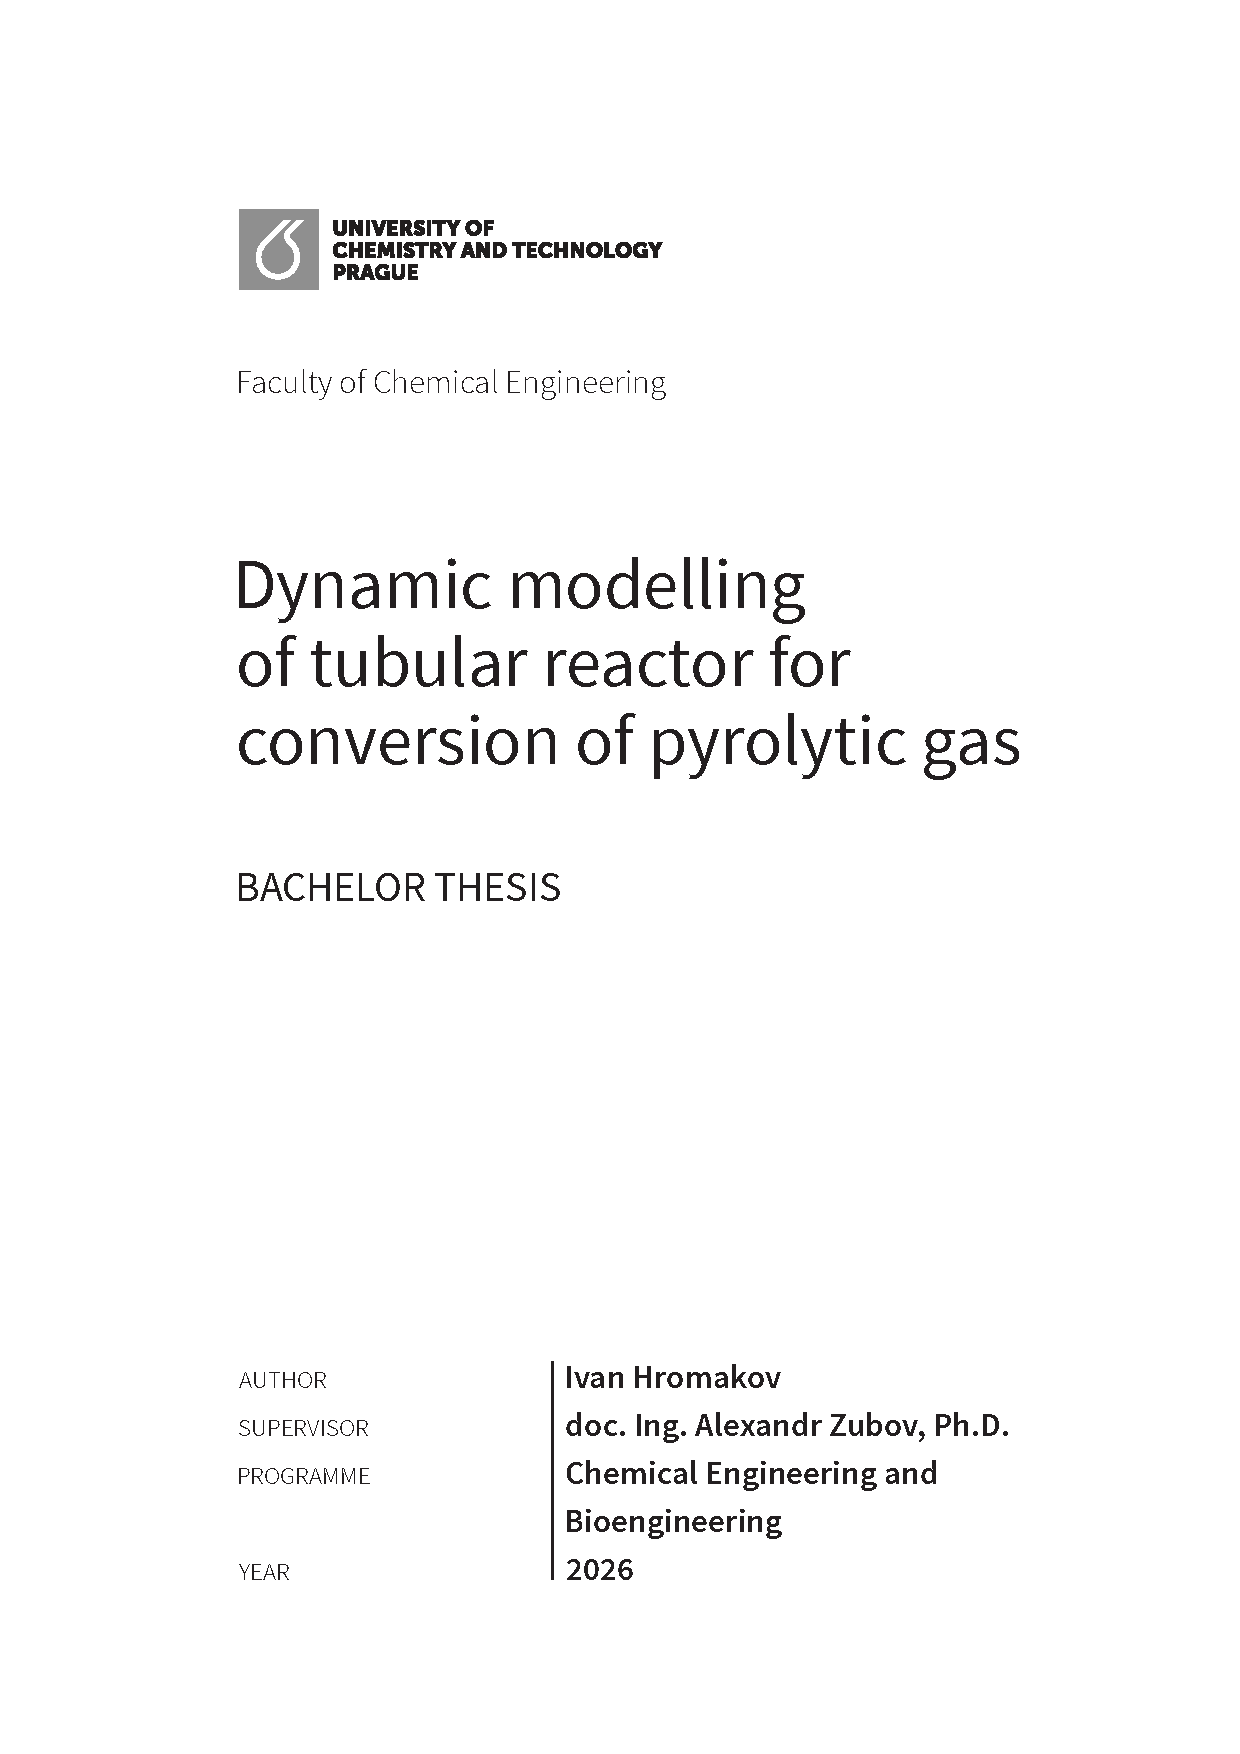
\includepdf[pages=-]{entry_sheet.pdf}

% =============================================================================
% FRONT MATTER — roman page numbering (i, ii, iii, ...)
% =============================================================================
\pagenumbering{roman}

% --- Summary (EN) and Souhrn (CZ) ---
% ===========================================================================
% chapters/summary.tex — Summary (EN) + Souhrn (CZ)
% ===========================================================================

\chapter*{Summary}
\addcontentsline{toc}{chapter}{Summary}
\markboth{SUMMARY}{SUMMARY}

This thesis develops a dynamic mathematical model of a non-catalytic tubular reformer that converts pyrolytic gas into hydrogen-rich syngas. The model combines a ten-species, eight-reaction lumped kinetic scheme with a one-dimensional plug-flow reactor discretised by first-order upwind finite volumes; nine side-stream injectors deliver oxygen and steam at staged positions along the reactor. Three time-integration algorithms --- forward Euler, backward Euler, and the variable-order integrator DLSODE --- are benchmarked on the resulting stiff convection--diffusion--reaction system. Parametric studies vary reactor temperature, inlet feed velocity, and side-injection flow rate; the results reveal a narrow but real operating window around the design point, with the side-injection flow-rate variation exhibiting a single optimum. Forward Euler at the default time step is identified as the cheapest integrator that meets the spatial-discretisation accuracy floor at the engineering-relevant grid; the recommendation is tied to the present isothermal kinetic scheme.

\selectlanguage{czech}

\chapter*{Souhrn}
\addcontentsline{toc}{chapter}{Souhrn}
\markboth{SOUHRN}{SOUHRN}

Tato práce vyvíjí dynamický matematický model nekatalytického trubkového reaktoru, který přeměňuje pyrolýzní plyn na syntézní plyn bohatý na vodík. Kinetické schéma s deseti složkami a osmi globálními reakcemi je spojeno s jednorozměrným modelem pístového reaktoru, prostorově diskretizovaným metodou konečných objemů s protisměrným schématem prvního řádu; podél osy reaktoru je rozmístěno devět bočních vstřiků dodávajících kyslík a vodní páru. Na vzniklém tuhém konvekčně-difúzně-reakčním systému jsou srovnány tři algoritmy časové integrace: explicitní Eulerova metoda, implicitní Eulerova metoda a integrátor DLSODE založený na metodě ``Backward Differentiation Formula'' (BDF) s proměnným řádem. Parametrické studie zkoumají vliv teploty reaktoru, vstupní rychlosti a průtoku bočních vstřiků; výsledky ukazují úzké, ale reálné provozní okno kolem pracovního bodu, přičemž variace průtoku bočních vstřiků vykazuje optimum. Doporučenou metodou je explicitní Eulerova metoda v jejím výchozím časovém kroku, která dosahuje přesnosti prostorové diskretizace na inženýrsky relevantní síti s nejnižšími výpočetními náklady; tato volba je vázána na použité izotermní kinetické schéma.

\selectlanguage{english}


% --- Table of Contents, List of Figures, List of Tables ---
\singlespacing%
\tableofcontents
\listoffigures
\listoftables
\newpage

% =============================================================================
% MAIN MATTER — arabic page numbering (1, 2, 3, ...)
% =============================================================================
\pagenumbering{arabic}
\onehalfspacing%

% --- Chapters ---
% ===========================================================================
% chapters/introduction.tex — Introduction
% ===========================================================================

\chapter*{Introduction}
\addcontentsline{toc}{chapter}{Introduction}
\markboth{INTRODUCTION}{INTRODUCTION}

Pyrolytic gas is a tar-laden by-product of the thermal treatment of solid waste streams: a hot mixture of methane, light hydrocarbons, aromatic intermediates, and combustion fragments that must be either reformed into a usable fuel or burned off. Reforming the tar component into hydrogen-rich syngas turns the waste stream into an industrial feedstock; an industrial interest in exactly this transformation motivated the present work. The reactor that does this is a non-catalytic tubular reformer operated near \SI{900}{\degreeCelsius}, with staged side-stream injection of oxygen and steam along its length. The thesis develops a dynamic mathematical model of this reactor, exercises it across an engineering operating envelope, and benchmarks three time-integration algorithms on the resulting stiff convection--diffusion--reaction system.

The chemistry of high-temperature thermal reforming is documented at two ends of the complexity spectrum: detailed elementary mechanisms with hundreds of species and thousands of reactions on one side, and single-lump cracking models with two or three pseudo-species on the other. Both are unsuitable for repeated reactor-scale simulation --- the first because of integration cost, the second because it cannot distinguish partial oxidation from steam reforming. This thesis adopts an intermediate lumped scheme of ten species and eight global reactions. The reactor model uses a finite-volume discretisation of the convection--diffusion--reaction equations on a one-dimensional plug-flow geometry, and the resulting semi-discrete system is benchmarked against three time-integration algorithms: forward Euler, backward Euler, and the variable-order Backward Differentiation Formula (BDF) integrator DLSODE.

The first chapter reviews the kinetic-model literature and selects the adopted eight-reaction scheme. The second develops the plug-flow reactor model and the first-order upwind finite-volume discretisation. The third assembles the full mathematical model and introduces the three time-integration algorithms. The fourth presents the engineering steady-state profiles, parametric studies, solver benchmarks, and a solver recommendation. The final chapter recaps the findings and identifies the next steps.

% =============================================================================
% chapters/kinetic_model.tex — Selection of the Kinetic Model
% =============================================================================
\chapter{Selection of the Kinetic Model}\label{ch:kinetic_model}

The kinetic model adopted in this work comprises 8 global reactions and approximately 10 species, employing three surrogate hydrocarbons: methane as a representative of aliphatic compounds, \(\alpha\)-methylstyrene as a representative of heavy aromatic tar, and benzene as an intermediate aromatic product. The model captures five distinct chemical phenomena: partial oxidation, steam reforming, hydrodealkylation, soot formation, and soot gasification.

Its design reflects the primary objective of the thesis: comparing numerical algorithms for solving reactor models based on their computational time, which requires a kinetic scheme that is complex enough to produce a meaningfully stiff system of equations, yet compact enough so that the chemistry does not dominate the total computation. To substantiate this choice, six alternative modelling approaches are reviewed below and evaluated against the criteria of computational tractability, physical fidelity, and suitability for algorithm benchmarking.

\section{Detailed elementary mechanisms}\label{sec:detailed_mechanisms}

Detailed kinetic mechanisms describe the reaction system at the level of individual elementary reactions. They explicitly track radical intermediates, pathways of polycyclic aromatic hydrocarbon (PAH) formation, and subsequent soot precursors. Such models aim to represent the underlying chemistry as comprehensively as possible. A well-known example is GRI-Mech~3.0~\cite{GRIMech}, originally developed for methane combustion. The mechanism contains 53 species and 325 reactions. However, it does not include aromatic species heavier than~\(\mathrm{C_3}\), which limits its applicability to tar conversion and PAH growth processes relevant for pyrolytic gas. More comprehensive mechanisms have been proposed for high-temperature aromatic chemistry. Norinaga \textit{et al.}~\cite{Norinaga2011} developed a Detailed Chemical Kinetic Model (DCKM) comprising more than 500 species and approximately 8\,000 elementary reactions. The model was validated against the experimental data of Jess~\cite{Jess1996} for benzene, toluene, and naphthalene conversion in tubular reactors at 800--1400~\si{\degreeCelsius}. Similarly, the CRECK mechanism by Ranzi \textit{et al.}~\cite{Ranzi2014} includes 509 species and 20\,240 reactions and was designed for coupled biomass pyrolysis and secondary gas-phase reactions. Although such mechanisms capture the relevant chemistry in great detail, they lead to large and stiff systems of equations with timescales spanning nanoseconds to seconds. Their solution requires implicit solvers with repeated Jacobian evaluations, and the computational cost increases rapidly with species number. As a result, integration times of hours to days make these mechanisms unsuitable for repeated simulations and algorithm benchmarking within the scope of this work.

\section{Skeletal and reduced mechanisms}\label{sec:skeletal_mechanisms}

Systematic reduction techniques such as the Directed Relation Graph (DRG) method and quasi-steady-state approximations yield skeletal mechanisms of 20--120 reactions. DRM-19 and DRM-22, reduced from GRI-Mech~\cite{GRIMech}, retain 19--22 species but contain no aromatics, tar, or soot chemistry. The Jones and Lindstedt~\cite{JonesLindstedt1988} 4-step global mechanism (\(\sim\)7 species, 4 reactions) is widely used in CFD for hydrocarbon combustion yet lacks any aromatic or soot pathway. A 39-species skeletal mechanism generates a Jacobian matrix approximately 25 times larger than the \(\sim\)10-species system of the adopted model, substantially increasing cost per integration step without contributing information relevant to the thesis objectives.

\section{Single-lump tar models}\label{sec:single_lump}

At the lower bound of complexity, single-lump models treat tar as one pseudo-species undergoing first-order thermal cracking. Boroson \textit{et al.}~\cite{Boroson1989} modelled wood pyrolysis tar as a single lump at 500--800~\si{\degreeCelsius}, and Fagbemi \textit{et al.}~\cite{Fagbemi2001} applied a similar one-reaction scheme (tar \(\to\) gas + soot) for three biomass types at 400--900~\si{\degreeCelsius}. With only 2--3 species and 1 reaction, these models can be numerically solved, but cannot distinguish partial oxidation from steam reforming and omit hydrodealkylation entirely.

\section{The adopted 8-reaction lumped model}\label{sec:adopted_model}

This model builds upon the work of Jess~\cite{Jess1996}, who reported global Arrhenius kinetics for the thermal conversion of naphthalene, toluene, and benzene in a tubular reactor at 700--1400~\si{\degreeCelsius} and \SI{160}{\kilo\pascal}, with activation energies of 247, 350, and \SI{493}{\kilo\joule\per\mole}, respectively. His experiments also showed strong inhibition of soot formation by hydrogen, while steam had only a minor direct effect on aromatic conversion rates.

In the present formulation, \(\alpha\)-methylstyrene is adopted as the heavy aromatic surrogate, replacing toluene and naphthalene. Three partial oxidation reactions~\eqref{eq:rxn1}--\eqref{eq:rxn3} use kinetic parameters from Smoot and Pratt~\cite{SmootPratt1979}, later validated for biomass-derived tar by Su \textit{et al.}~\cite{Su2011}. Methane steam reforming~\eqref{eq:rxn4} follows Jones and Lindstedt~\cite{JonesLindstedt1988}; benzene steam reforming with soot formation~\eqref{eq:rxn5} and soot gasification~\eqref{eq:rxn8} are taken from Jess~\cite{Jess1996}; and \(\alpha\)-methylstyrene steam reforming~\eqref{eq:rxn6} together with hydrodealkylation~\eqref{eq:rxn7} are based on Taralas \textit{et al.}~\cite{Taralas2003}. Umeki \textit{et al.}~\cite{Umeki2012} further demonstrated that a closely related reduced scheme provides satisfactory predictions for biomass gasification.

The resulting \(\sim\)10-species, 8-reaction system forms a coupled and stiff problem, where fast partial oxidation competes with much slower steam reforming reactions. This creates a computational regime in which the choice of numerical method (explicit vs.\ implicit, adaptive vs.\ fixed step) has a measurable impact on solution time, making the model suitable for a numerical algorithm comparison.

\section{Multi-component tar models}\label{sec:multicomponent}

Multi-component approaches track 4--13 individual tar species classified according to the Evans and Milne~\cite{EvansMilne1987} maturation scheme (primary oxygenates through condensed tertiary PAHs). Morf \textit{et al.}~\cite{Morf2002} provided detailed experimental characterisation of homogeneous secondary tar reactions in a tubular reactor at 500--1000~\si{\degreeCelsius}. Salem \textit{et al.}~\cite{Salem2019} implemented 4 tar species with 18 reactions in a downdraft gasifier model, noting that benzene, naphthalene, toluene, and phenol together represent 70--95\,\% of all tar species. Fuentes-Cano \textit{et al.}~\cite{FuentesCano2016} developed a lumped tar-class model that quantitatively predicts tar yields at 700--1000~\si{\degreeCelsius}. Dufour \textit{et al.}~\cite{Dufour2011} established that \ce{CH4} production is controlled primarily by aromatic demethylation --- a finding that directly supports the hydrodealkylation pathway (reaction~\eqref{eq:rxn7}) in the adopted model. These multi-component schemes (15--30 species, 18--27 reactions) provide improved tar speciation at 3--10 times the computational cost of the 8-reaction model, an overhead that is justified for process design but counterproductive for numerical algorithm benchmarking.

\section{Equilibrium models}\label{sec:equilibrium}

Thermodynamic equilibrium models based on Gibbs free energy minimisation predict zero tar at all gasification temperatures, since aromatic hydrocarbons are thermodynamically unstable above approximately \SI{600}{\degreeCelsius}. In practice, tar persists because its destruction is kinetically controlled: typical residence times of 1--5~s at \SI{900}{\degreeCelsius} are insufficient for complete conversion. Equilibrium approaches also overestimate \ce{H2} and \ce{CO} yields by 10--50\,\% and underestimate \ce{CH4}. Modified approaches such as the constrained free energy method of Kangas \textit{et al.}~\cite{Kangas2014} partially address these shortcomings by introducing empirical corrections, but in doing so sacrifice the generality that constitutes equilibrium modelling's principal advantage. More fundamentally, equilibrium models contain no time dimension and are therefore incompatible with the dynamic, non-isothermal tubular reactor framework of this thesis.

\section{Empirical and data-driven models}\label{sec:empirical}

Empirical correlations and machine learning models relate product yields directly to operating parameters. While computationally inexpensive, they provide no mechanistic insight, cannot extrapolate beyond their calibration range, and --- critically --- contain no differential equations. They are therefore irrelevant to a thesis concerned with comparing various numerical solvers suitable for modelling of dynamics in a tubular reactor.

\section{Summary}\label{sec:kinetic_conclusion}

The 8-reaction lumped model represents the minimum-complexity kinetic framework that captures the complete phenomenology of non-catalytic thermal reforming at \(\sim\)\SI{900}{\degreeCelsius}. Models of lower complexity (equilibrium, single-lump, empirical) sacrifice essential physics: equilibrium cannot predict tar; single-lump schemes omit hydrodealkylation and partial oxidation selectivity; empirical models contain no equations to solve. Models of higher complexity (skeletal, detailed) introduce chemical detail that, while scientifically valuable, would dominate total computation time and obscure the numerical algorithm comparison that constitutes the thesis's core contribution. The literature confirms that lumped kinetic models at this level of complexity --- validated by Jess~\cite{Jess1996}, extended by Umeki \textit{et al.}~\cite{Umeki2012}, and corroborated by the tar-class work of Fuentes-Cano \textit{et al.}~\cite{FuentesCano2016} and the review of Savage~\cite{Savage2000} --- provide predictions sufficiently accurate for reactor-scale simulation while remaining computationally tractable for systematic solver benchmarking.

\section{Kinetic Rate Expressions}\label{sec:kinetic_rates}

\subsection{Partial oxidation reactions}\label{ssec:partial_oxidation}

The partial oxidation kinetics follow the global scheme of Smoot and Pratt~\cite{SmootPratt1979}. The original kinetic data were derived from coal pyrolysis gas containing \SI{42.3}{\mole\percent} methane with the remainder consisting of other (unspecified) hydrocarbons. The activation energy of hydrocarbon oxidation in this framework ranges from 80 to \SI{150}{\kilo\joule\per\mole}, and the reaction order with respect to the hydrocarbon species ranges from 0.5 to~1. It is assumed that all three surrogate hydrocarbons react with oxygen at comparable rates.

The generalised reaction is
%
\begin{equation}
  \ce{C_{n}H_{m}} + \frac{n}{2}\,\ce{O2} \longrightarrow n\,\ce{CO} + \frac{m}{2}\,\ce{H2}
  \label{eq:gen_partial_ox}
\end{equation}
%
with Arrhenius-type rate expression
%
\begin{equation}
  r_i = A_i \exp\!\Bigl(-\frac{E_i}{RT}\Bigr)\,[\text{fuel}]\,[\ce{O2}]
  \label{eq:partial_ox_rate}
\end{equation}

\paragraph{Methane partial oxidation.}
%
\begin{equation}
  \ce{CH4 + \frac{1}{2} O2 -> CO + 2 H2}
  \label{eq:rxn1}
\end{equation}
%
Using the parameters for long-chain hydrocarbons:
%
\begin{align}
  A_1 &= \SI{59.8}{\metre\cubed\per\mole\per\second} \label{eq:A1} \\
  E_1 &= \SI{101.4}{\kilo\joule\per\mole}. \label{eq:E1}
\end{align}

\paragraph{Benzene partial oxidation.}
%
\begin{equation}
  \ce{C6H6 + 3 O2 -> 6 CO + 3 H2}
  \label{eq:rxn2}
\end{equation}
%
Using cyclic hydrocarbon parameters:
%
\begin{align}
  A_2 &= \SI{2.07e4}{\metre\cubed\per\mole\per\second} \label{eq:A2} \\
  E_2 &= \SI{80.2}{\kilo\joule\per\mole}. \label{eq:E2}
\end{align}

\paragraph{\(\alpha\)-Methylstyrene partial oxidation.}
%
\begin{equation}
  \ce{C9H10 + \frac{9}{2} O2 -> 9 CO + 5 H2}
  \label{eq:rxn3}
\end{equation}
%
Assuming aromatic behaviour consistent with cyclic hydrocarbons:
%
\begin{align}
  A_3 &= \SI{2.07e4}{\metre\cubed\per\mole\per\second} \label{eq:A3} \\
  E_3 &= \SI{80.2}{\kilo\joule\per\mole}. \label{eq:E3}
\end{align}

\subsection{Steam reforming of methane}\label{ssec:steam_reforming_CH4}

The steam reforming of methane is represented by the global reaction
%
\begin{equation}
  \ce{CH4 + H2O -> CO + 3 H2}
  \label{eq:rxn4}
\end{equation}

Jones and Lindstedt~\cite{JonesLindstedt1988} determined the kinetics of alkane reactions in a mixture with air by analysing the flame structure. While the oxidation kinetics derived from flame conditions cannot be directly applied to a tubular reformer model, the steam reforming kinetics remain transferable, as the underlying gas-phase fuel breakdown chemistry is not specific to the flame environment. In general, the steam reforming reaction is many times slower than partial oxidation, and light hydrocarbons react more readily with steam than do aromatic species.

For methane (\(n = 1\)), the forward rate is given by
%
\begin{equation}
  r_4 = k_4(T)\,[\ce{CH4}]\,[\ce{H2O}]
  \label{eq:rate4}
\end{equation}
%
with the Arrhenius temperature dependence
%
\begin{equation}
  k_4(T) = A_4\, T^{b_4} \exp\!\Bigl(-\frac{E_4}{RT}\Bigr).
  \label{eq:k4}
\end{equation}
%
For methane, the kinetic parameters are
%
\begin{align}
  A_4 &= \SI{3.0e8}{\metre\cubed\per\mole\per\second} \label{eq:A4} \\
  b_4 &= 0 \label{eq:b4} \\
  E_4 &= \SI{30000}{cal\per\mole}, \label{eq:E4_cal}
\end{align}
%
which corresponds to an activation energy of
%
\begin{equation}
  E_4 = \SI{125.5}{\kilo\joule\per\mole}.
  \label{eq:E4}
\end{equation}

The reaction is first order with respect to methane and first order with respect to steam, resulting in an overall second-order rate expression, consistent with the general observation that steam reforming of light hydrocarbons follows second-order kinetics. This kinetic formulation represents a global gas-phase fuel breakdown step calibrated for high-temperature flame conditions rather than a catalytic steam reforming mechanism.

\subsection{Steam reforming of benzene}\label{ssec:steam_reforming_benzene}

The steam reforming of benzene with concurrent soot formation is represented by
%
\begin{equation}
  \ce{C6H6 + 2 H2O -> 2 CO + \frac{5}{2} CH4 + \frac{3}{2} C}
  \label{eq:rxn5}
\end{equation}
%
Jess~\cite{Jess1996} reported an activation energy of \SI{493}{\kilo\joule\per\mole} for the steam reforming of benzene; however, the value used in the present model is reduced by \SI{50}{\kilo\joule\per\mole} to \SI{443}{\kilo\joule\per\mole}. This adjustment is necessary because, with the original activation energy, the reaction does not proceed in the model and no soot is formed, which contradicts the experimental observation that soot formation does occur under the relevant conditions. The modification falls within the accepted uncertainty range of \(\pm\SI{100}{\kilo\joule\per\mole}\) for global kinetic parameters of this type. This reaction constitutes the sole pathway for soot formation in the model. At a temperature of \SI{900}{\degreeCelsius} and in the absence of polycyclic aromatic hydrocarbons (naphthalene, pyrene), a large amount of soot is not expected, but it cannot be completely neglected. The steam reforming of aromatic species follows approximately first-order kinetics with respect to the aromatic concentration (the fitted exponent for benzene is~1.3, see \cref{eq:rate5}), in contrast to the second-order dependence observed for light hydrocarbons.

%
The global rate expression for benzene conversion is
%
\begin{equation}
  r_5 = k_5(T)\,{[\ce{C6H6}]}^{1.3}\,{[\ce{H2}]}^{-0.4}\,{[\ce{H2O}]}^{0.2}
  \label{eq:rate5}
\end{equation}
%
with
%
\begin{equation}
  k_5(T) = A_5 \exp\!\Bigl(-\frac{E_5}{RT}\Bigr)
  \label{eq:k5}
\end{equation}
%
and kinetic parameters
%
\begin{align}
  A_5 &= \SI{2.0e16}{\mole^{-0.1}\,\metre^{0.3}\,\per\second} \label{eq:A5} \\
  E_5 &= \SI{443}{\kilo\joule\per\mole}. \label{eq:E5}
\end{align}

The reaction exhibits a strong temperature dependence and a weak positive dependence on steam concentration, while hydrogen inhibits benzene conversion.

\subsection{Steam reforming of \texorpdfstring{\(\alpha\)}{alpha}-methylstyrene}\label{ssec:steam_reforming_AMS}

The steam reforming of the heavy aromatic surrogate is represented by
%
\begin{equation}
  \ce{C9H10 + 11.5 H2O -> 6.5 CO + 2.5 CO2 + 16.5 H2}
  \label{eq:rxn6}
\end{equation}

Taralas \textit{et al.}~\cite{Taralas2003} investigated thermal destruction of toluene in a tubular flow reactor at 973--1223~K under conditions similar to those of the present model. This reaction is the only source of \ce{CO2} in the model. In the original study, equal stoichiometric amounts of \ce{CO} and \ce{CO2} are formed. The stoichiometry adopted here was adjusted so that less \ce{CO2} is produced, in order to match the gas composition obtained from thermodynamic equilibrium calculations in Aspen Plus. This adjustment compensates for the absence of the reverse water-gas shift reaction in the model. Assuming first-order dependence with respect to the aromatic species and excess steam conditions, the rate expression is written as

%
\begin{equation}
  r_6 = k_6(T)\,[\ce{C9H10}]
  \label{eq:rate6}
\end{equation}
%
with Arrhenius temperature dependence
%
\begin{equation}
  k_6(T) = A_6 \exp\!\Bigl(-\frac{E_6}{RT}\Bigr)
  \label{eq:k6}
\end{equation}
%
where
%
\begin{align}
  A_6 &= \SI{2.3e15}{\per\second} \label{eq:A6} \\
  E_6 &= \SI{356}{\kilo\joule\per\mole}. \label{eq:E6}
\end{align}

The high activation energy reflects the refractory nature of aromatic steam reforming reactions.

\subsection{Hydrodealkylation of \texorpdfstring{\(\alpha\)}{alpha}-methylstyrene}\label{ssec:hydrodealkylation}

Hydrodealkylation is described by
%
\begin{equation}
  \ce{C9H10 + 4 H2 -> 3 CH4 + C6H6}
  \label{eq:rxn7}
\end{equation}
%
Taralas \textit{et al.}~\cite{Taralas2003} studied toluene destruction under both oxidative and reducing atmospheres at conditions similar to those of the present model. The rate expression follows a first-order dependence on the aromatic species and half-order dependence on the hydrogen-containing mixture:

%
\begin{equation}
  r_7 = k_7(T)\,[\ce{C9H10}]\,{[\ce{H2}]}^{0.5}
  \label{eq:rate7}
\end{equation}
%
with Arrhenius form
%
\begin{equation}
  k_7(T) = A_7 \exp\!\Bigl(-\frac{E_7}{RT}\Bigr)
  \label{eq:k7}
\end{equation}
%
and kinetic parameters
%
\begin{align}
  A_7 &= \SI{3.3e10}{\mole^{-0.5}\,\metre^{1.5}\,\per\second} \label{eq:A7} \\
  E_7 &= \SI{250}{\kilo\joule\per\mole}. \label{eq:E7}
\end{align}

The presence of hydrogen lowers the activation energy by approximately \SI{100}{\kilo\joule\per\mole} compared to steam reforming conditions, leading to significantly faster aromatic conversion.

\subsection{Soot gasification}\label{ssec:soot_gasification}

The heterogeneous gasification of soot is described by
%
\begin{equation}
  \ce{C + H2O -> CO + H2}
  \label{eq:rxn8}
\end{equation}

Because soot is a solid phase, the volumetric rate depends on both the steam concentration and the local soot mass concentration \(\rho_{\mathrm{soot}}\)~\([\si{\kilogram\per\metre\cubed}]\):
%
\begin{equation}
  r_8 = k_8(T)\,\rho_{\mathrm{soot}}\,[\ce{H2O}]
  \label{eq:rate8}
\end{equation}
%
with Arrhenius dependence
%
\begin{equation}
  k_8(T) = A_8 \exp\!\Bigl(-\frac{E_8}{RT}\Bigr).
  \label{eq:k8}
\end{equation}
%
The kinetic parameters determined by Jess~\cite{Jess1996} are
%
\begin{align}
  A_8 &= \SI{3.0e11}{\metre\cubed\,\per\kilogram\,\per\second} \label{eq:A8} \\
  E_8 &= \SI{310}{\kilo\joule\per\mole}. \label{eq:E8}
\end{align}

The soot gasification step is first order with respect to steam and strongly temperature dependent. Because this reaction is slow relative to the other steps in the model, sufficient excess steam must be supplied to the reactor for the gasification of deposited soot to proceed at a meaningful rate. Without adequate steam, any soot formed by reaction~\eqref{eq:rxn5} would accumulate along the reactor length.

% ===========================================================================
% chapters/governing_equations.tex — Governing Equations and Finite Volume
%                                     Discretisation
% ===========================================================================

\chapter{Tubular Reactor Model and Spatial Discretisation}\label{ch:governing_eqs}

This chapter develops the mathematical framework that connects the kinetic model of \cref{ch:kinetic_model} to a numerically tractable system. The convection-diffusion-reaction equation governing species transport in a plug flow reactor (PFR) is first derived from mass conservation principles. The partial differential equation is then discretised in space using the finite volume method (FVM), yielding a system of ordinary differential equations suitable for the time integration methods studied in subsequent chapters. Particular emphasis is placed on the conservation properties of FVM and their physical significance for the reactive flow problem.

\section{The Plug Flow Reactor Model}\label{sec:pfr_model}

The reactor is modelled as a one-dimensional tube of length~\(L\) and constant cross-sectional area~\(A\), following the standard axial dispersion model~\cite{Levenspiel1999, Froment2011}. The gaseous reaction mixture flows at superficial velocity~\(u\) along the axial coordinate~\(x \in [0, L]\). The following assumptions reduce the three-dimensional transport problem to a single spatial dimension:

%
\begin{itemize}
  \item Radial concentration and temperature gradients are negligible.
  \item The flow is axially symmetric --- no angular variation.
  \item The overall pressure is approximately constant along the reactor.
  \item The cross-sectional area of the reactor is constant.
\end{itemize}

Under these conditions, the molar concentration~\(C_i(x,t)\) of species~\(i\) is governed by the one-dimensional species transport equation

%
\begin{equation}
  \frac{\partial C_i}{\partial t}
  + u\,\frac{\partial C_i}{\partial x}
  = \Dax\,\frac{\partial^2 C_i}{\partial x^2}
  + \Ri
  \label{eq:species_transport}
\end{equation}
%

where

%
\begin{itemize}
  \item \(C_i\) is the molar concentration of species~\(i\)
        \([\si{\mole\per\metre\cubed}]\),
  \item \(u\) is the superficial gas velocity \([\si{\metre\per\second}]\),
  \item \(\Dax\) is the axial dispersion coefficient
        \([\si{\metre\squared\per\second}]\),
  \item \(\Ri\) is the net volumetric rate of production of
        species~\(i\) \([\si{\mole\per\metre\cubed\per\second}]\), computed
        from the rate expressions developed in
        \cref{ch:kinetic_model}.
\end{itemize}

The four terms in \cref{eq:species_transport} have distinct physical meanings. The first term on the left-hand side, \(\partial C_i / \partial t\), represents the local accumulation of species~\(i\). The second term, \(u\,\partial C_i / \partial x\), describes convective transport --- the bulk gas flow carries species downstream. On the right-hand side, the dispersion term \(\Dax\,\partial^2 C_i / \partial x^2\) accounts for axial spreading caused by turbulent mixing and molecular diffusion. The source term \(R_i\) couples the transport equation to the chemical kinetics of \cref{ch:kinetic_model}.

\subsection{Boundary and Initial Conditions}\label{ssec:boundary_conditions}

At the reactor inlet (\(x = 0\)), a Danckwerts boundary condition~\cite{Danckwerts1953} balances the convective and diffusive fluxes:

%
\begin{equation}
  u\,C_i\big|_{x=0^-}
  = u\,C_i\big|_{x=0^+}
  - \Dax\,\frac{\partial C_i}{\partial x}\bigg|_{x=0^+}
  \label{eq:danckwerts_inlet}
\end{equation}
%

For the idealised PFR, where axial dispersion is small (\(\Dax \to 0\)), this reduces to a Dirichlet condition:
%
\begin{equation}
  C_i(0, t) = \Cin(t)
  \label{eq:dirichlet_inlet}
\end{equation}
%
At the reactor outlet (\(x = L\)), a zero-gradient (Neumann) condition represents fully developed flow with no diffusive flux leaving the domain:
%
\begin{equation}
  \frac{\partial C_i}{\partial x}\bigg|_{x=L} = 0
  \label{eq:neumann_outlet}
\end{equation}
%
The initial condition specifies the concentration distribution at \(t = 0\):
%
\begin{equation}
  C_i(x, 0) = C_{i,0}(x)
  \label{eq:initial_condition}
\end{equation}
%
\subsection{The P\'eclet Number and Convection Dominance}\label{ssec:peclet}

The relative importance of convective and diffusive transport is characterised by the P\'eclet number:
%
\begin{equation}
  \Pe = \frac{u\,L}{\Dax}
  \label{eq:peclet}
\end{equation}
%
which represents the ratio of the convective transport rate to the diffusive transport rate. For tubular reactors the axial dispersion coefficient \(\Dax\) must be estimated from the flow regime. In the laminar regime (\(\Re < 2100\)), the Aris-Taylor analysis~\cite{Taylor1953, Aris1956} gives
%
\begin{equation}
  \Dax = D_{AB} + \frac{u^2\,R^2}{48\,D_{AB}},
  \label{eq:aris_taylor}
\end{equation}
%
where \(D_{AB}\) is the molecular diffusivity and \(R\) the tube radius. For the turbulent and transitional regimes, Fogler~\cite{Fogler2006} (Chapter~14, Figures~14-10 and 14-11, pp.~964--965) summarises experimental correlations giving the dimensionless dispersion number \(\Dax/(u\,d_t)\) as a function of the Reynolds and Schmidt numbers. For typical tubular reactors at high temperature, P\'eclet numbers of order \(10^3\) to \(10^5\) can be inferred from these correlations~\cite{Fogler2006, Levenspiel1999, Froment2011}, indicating strong convection dominance. This has two important consequences.

First, the species concentration profile develops a steep front that propagates downstream with the flow, and diffusion plays only a minor smoothing role.

Second, the choice of numerical scheme for the convective term becomes critical: naive central differencing produces unphysical oscillations when convection dominates, as will be discussed in \cref{ssec:convective_flux}.

In the limiting case \(\Pe \to \infty\), the dispersion term vanishes entirely and \cref{eq:species_transport} reduces to the pure convection-reaction equation of an ideal PFR\@.

\section{Finite Volume Discretisation}\label{sec:fvm}

The finite volume method converts the partial differential \cref{eq:species_transport} into a system of ordinary differential equations by dividing the reactor into discrete control volumes and enforcing mass conservation over each one. The key advantage of FVM is that conservation is guaranteed by construction --- the method is derived directly from the integral form of the conservation law, as explained below.

\subsection{The CSTR Cascade Approximation}\label{ssec:cstr_cascade}

Before systematic spatial discretisation techniques such as FVM became standard in chemical engineering practice, plug flow behaviour was commonly approximated by connecting \(N\) ideally mixed continuous stirred tank reactors (CSTRs) in series~\cite{Kosek2022, Levenspiel1999}. Each tank in the cascade has identical volume \(V\) and is fed at a constant volumetric flow rate \(\dot V\), so that its mean residence time is \(\tau = V/\dot V\). For an inert tracer, the molar balance of species \(A\) in the \(i\)-th tank reads
%
\begin{equation}
  \frac{\mathrm{d}c_{A,i}}{\mathrm{d}t}
  = \frac{1}{\tau}\,\bigl(c_{A,i-1} - c_{A,i}\bigr),
  \qquad i = 1,\,\ldots,\,N,
  \label{eq:cstr_cascade_balance}
\end{equation}
%
with \(c_{A,0}(t)\) prescribing the inlet concentration to the first tank. The hydrodynamic character of this idealised cascade is conventionally analysed through its residence time distribution (RTD), introduced by Danckwerts~\cite{Danckwerts1953}. For a Dirac pulse injected at the inlet, the differential RTD function at the outlet of the cascade is~\cite{Kosek2022, Levenspiel1999}
%
\begin{equation}
  E(t)
  = \frac{t^{N-1}}{(N-1)!}\,
    {\left(\frac{N}{\tau}\right)}^{N}\,
    \exp\!\left(-\frac{N\,t}{\tau}\right),
  \label{eq:rtd_cascade}
\end{equation}
%
which is a Gamma distribution of shape parameter~\(N\). The full derivation proceeds by integrating \cref{eq:cstr_cascade_balance} for a tracer pulse and is given in~\cite{Kosek2022}. For \(N = 1\), \cref{eq:rtd_cascade} reduces to the familiar exponential decay \(E(t) = (1/\tau)\exp(-t/\tau)\) of a single perfectly mixed tank. As \(N\) grows, the distribution narrows into a peak that is centred at \(t = \tau\), and in the limit \(N \to \infty\) it approaches the Dirac delta \(\delta(t - \tau)\), corresponding to the complete absence of axial mixing --- that is, ideal plug flow. \cref{fig:rtd_cascade} illustrates this convergence for several values of~\(N\).

\begin{figure}[H]
\centering
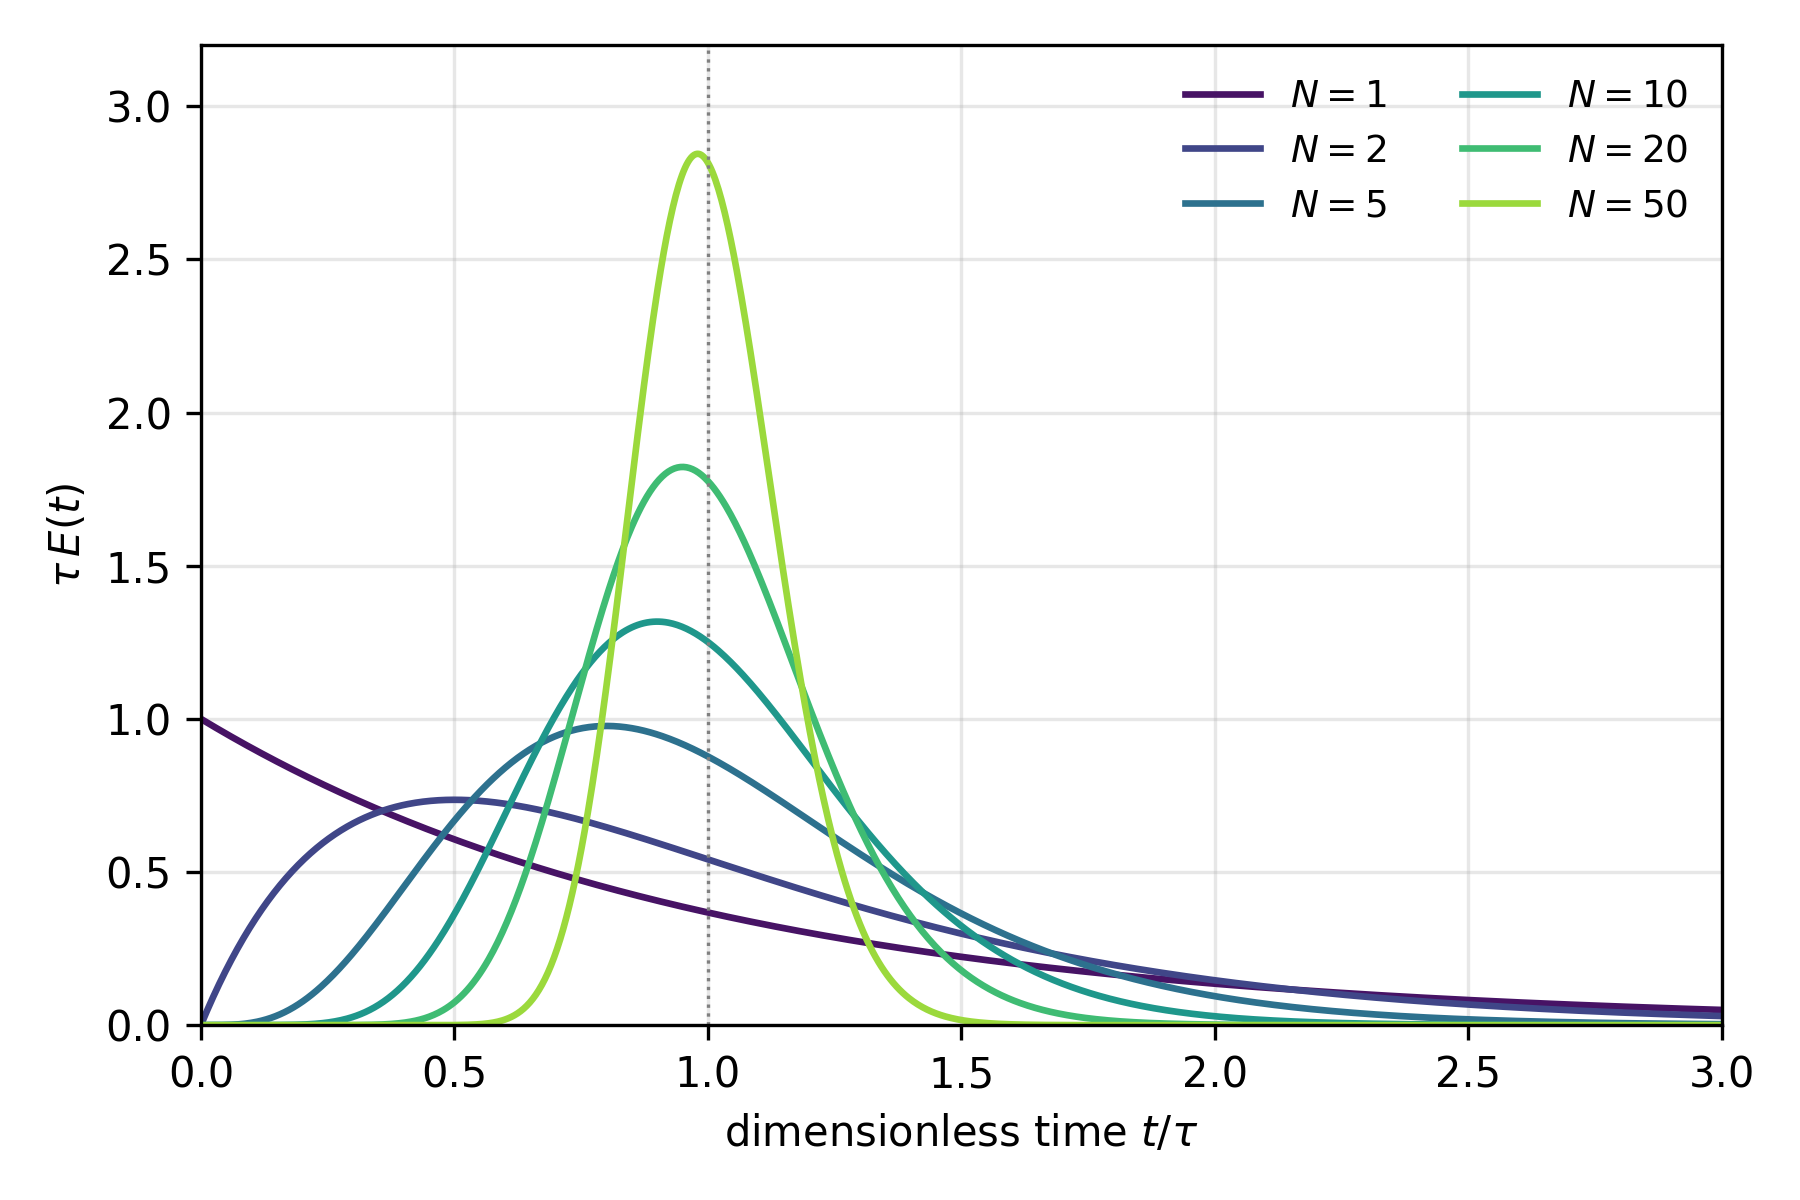
\includegraphics[width=0.68\textwidth]{figures/rtd_cascade.png}
\caption{Differential residence time distribution function \(E(t)\), shown in
the dimensionless form \(\tau\,E(t)\) versus \(t/\tau\), for a cascade of
\(N\) ideally mixed CSTRs. As \(N\) increases, the distribution narrows around
the mean residence time, and in the limit \(N \to \infty\) it converges to the
Dirac delta of an ideal plug flow reactor.}\label{fig:rtd_cascade}
\end{figure}
\FloatBarrier

The finite volume method developed in the remainder of this chapter can be viewed as a formal generalisation of this older engineering intuition. In FVM the reactor domain is partitioned into \(N\) computational cells, each of which carries a single cell-averaged concentration --- effectively the assumption that the field is well mixed within the cell. 

The first-order upwind flux introduced in \cref{ssec:convective_flux} mirrors the cascade construction exactly: the convective flux leaving cell~\(j\) is evaluated using the concentration \emph{inside} that cell, just as the outlet stream of a CSTR carries its own well-mixed tank concentration to the next reactor in the series. Mesh refinement, i.e.\ increasing the number of cells, is the spatial counterpart of adding more tanks to the cascade, and the limit \(N \to \infty\) recovers ideal plug flow in both formulations. 

The cascade picture thus provides a direct physical interpretation of why an ostensibly piecewise-constant discretisation is a sensible approximation for a convection-dominated tubular reactor, and it motivates the systematic conservative derivation of the FVM equations that follows.

\subsection{The Integral Conservation Law}\label{ssec:conservation_law}

The species transport \cref{eq:species_transport} is the differential form of a more fundamental statement: the integral conservation law~\cite{LeVeque2002}. For any \emph{spatial} interval \([a,\,b]\) along the reactor axis, mass conservation of species~\(i\) requires
%
\begin{equation}
  \frac{\mathrm{d}}{\mathrm{d}t}
  \int_a^b C_i\,\mathrm{d}x
  = F_i\big|_{x=a} - F_i\big|_{x=b}
  + \int_a^b R_i\,\mathrm{d}x
  \label{eq:integral_conservation}
\end{equation}
%
where \(F_i = u\,C_i - \Dax\,\partial C_i / \partial x\) is the total (convective plus diffusive) flux of species~\(i\) in the positive \(x\)-direction. In other words: the rate of change of the total amount of species~\(i\) between \(a\) and~\(b\) equals the flux entering through the left face minus the flux leaving through the right face, plus the amount produced by chemical reactions within the interval. 

This is a direct expression of mass conservation. Unlike the spatial form~\eqref{eq:species_transport}, which requires the concentration field to be sufficiently smooth, the integral form~\eqref{eq:integral_conservation} remains valid even at discontinuities such as sharp concentration fronts that are common in convection-dominated flows~\cite{LeVeque2002}. 

The finite volume method, as described by Versteeg and Malalasekera~\cite{Versteeg2007} and LeVeque~\cite{LeVeque2002}, discretizes the integral form~\eqref{eq:integral_conservation} directly. Each computational cell occupying interval \([x_{j-1/2},\, x_{j+1/2}]\) is itself a control volume, and the discrete equation for that cell is a conservation statement.

\newpage
A crucial consequence is the \emph{telescoping property}: the flux leaving cell~\(j\) through face~\(j + \tfrac{1}{2}\) is identical to the flux entering cell~\(j{+}1\) through the same face. When the discrete equations for all cells are summed, the internal fluxes cancel exactly, and only the boundary fluxes at \(x = 0\) and \(x = L\) remain. 

This means that the total amount of species in the reactor can change only through the inlet and outlet boundaries or through chemical reaction --- the discretisation itself neither creates nor destroys mass. For the plug flow reactor, this property has a direct physical interpretation: every mole of a species that leaves one control volume enters the next. 

The stoichiometric relationships established by the kinetic model in \cref{ch:kinetic_model} are preserved at the discrete level. Methods that start from the differential form, such as the finite difference method, do not automatically guarantee this cell-by-cell balance and may introduce small but systematic mass conservation errors over long integration times.

\subsection{Domain Decomposition into Control Volumes}\label{ssec:control_volumes}

The reactor domain \([0, L]\) is divided into \(N\) non-overlapping control volumes (cells). Cell~\(j\) occupies the interval \([x_{j-1/2},\, x_{j+1/2}]\) with cell centre~\(x_j\) and width \(\Delta x_j = x_{j+1/2} - x_{j-1/2}\). For a uniform grid, \(\Delta x = L / N\) and \(x_j = (j - \tfrac{1}{2})\,\Delta x\).

%
\begin{figure}[H]
\centering
\begin{tikzpicture}[>=stealth, thick, scale=1.25, every node/.style={scale=1.0}]
  % Flow arrow
  \draw[->, very thick, blue!70!black] (-0.5, 1.8) -- (2.0, 1.8)
    node[midway, above] {\(u\)};
  % Cells
  \foreach \j/\lab in {0/{j{-}1}, 3.5/{j}, 7/{j{+}1}} {
    \draw (\j, 0) rectangle (\j+3.5, 1.2);
    \node at (\j+1.75, 0.6) {\(\bar{C}_{i,\lab}\)};
  }
  % Cell centres
  \foreach \j/\lab in {1.75/{j{-}1}, 5.25/{j}, 8.75/{j{+}1}} {
    \fill (\j, 0) circle (2pt);
    \node[below=4pt] at (\j, 0) {\(x_{\lab}\)};
  }
  % Face labels
  \foreach \j/\lab in {3.5/{j{-}\frac{1}{2}}, 7/{j{+}\frac{1}{2}}} {
    \draw[dashed, gray] (\j, -0.3) -- (\j, 1.5);
    \node[above=2pt] at (\j, 1.2) {\(x_{\lab}\)};
  }
  % Flux arrows (below cells to avoid overlap)
  \draw[->, red!70!black, thick] (2.5, -0.4) -- (4.5, -0.4)
    node[midway, below=2pt] {\(F_{j-\frac{1}{2}}\)};
  \draw[->, red!70!black, thick] (6.0, -0.4) -- (8.0, -0.4)
    node[midway, below=2pt] {\(F_{j+\frac{1}{2}}\)};
  % Delta x brace
  \draw[decorate, decoration={brace, amplitude=5pt, mirror}]
    (3.5, -1.2) -- (7, -1.2)
    node[midway, below=6pt] {\(\Delta x\)};
\end{tikzpicture}

\caption{One-dimensional uniform control volume mesh. Cell~\(j\) is bounded by
faces at \(x_{j-1/2}\) and \(x_{j+1/2}\). The cell-averaged concentration
\(\bar{C}_{i,j}\) is stored at the cell centre~\(x_j\). Fluxes \(F\) are
evaluated at each face.}\label{fig:control_volume}
\end{figure}

The unknown quantity in each cell is the cell-averaged concentration:

%
\begin{equation}
  \bar{C}_{i,j}(t)
  = \frac{1}{\Delta x}
    \int_{x_{j-1/2}}^{x_{j+1/2}} C_i(x,t)\,\mathrm{d}x
  \label{eq:cell_average}
\end{equation}
%

\subsection{Integration Over a Control Volume}\label{ssec:fvm_integration}

Integrating \cref{eq:species_transport} over cell~\(j\) gives
%
\begin{equation}
  \int_{x_{j-1/2}}^{x_{j+1/2}}
    \frac{\partial C_i}{\partial t}\,\mathrm{d}x
  + \int_{x_{j-1/2}}^{x_{j+1/2}}
    \frac{\partial\,(u\,C_i)}{\partial x}\,\mathrm{d}x
  = \int_{x_{j-1/2}}^{x_{j+1/2}}
    \Dax\,\frac{\partial^2 C_i}{\partial x^2}\,\mathrm{d}x
  + \int_{x_{j-1/2}}^{x_{j+1/2}} R_i\,\mathrm{d}x
  \label{eq:fvm_integral}
\end{equation}

Applying the fundamental theorem of calculus to the convective and diffusive integrals converts them from volume integrals to surface (face) evaluations:
%
\begin{equation}
  \Delta x\,\frac{\mathrm{d}\bar{C}_{i,j}}{\mathrm{d}t}
  + {\Bigl[u\,C_i\Bigr]}_{x_{j-1/2}}^{x_{j+1/2}}
  = {\biggl[\Dax\,
    \frac{\partial C_i}{\partial x}\biggr]}_{x_{j-1/2}}^{x_{j+1/2}}
  + \Delta x\,\bar{R}_{i,j}
  \label{eq:fvm_semidiscrete_raw}
\end{equation}

The convective and diffusive contributions at each face are collected into fluxes. The convective flux at face \(j + \tfrac{1}{2}\) is
%
\begin{equation}
  F^{\mathrm{c}}_{j+1/2} = u\,C_i\big|_{x_{j+1/2}}
  \label{eq:convective_flux}
\end{equation}
%
and the diffusive flux is
%
\begin{equation}
  F^{\mathrm{d}}_{j+1/2}
  = -\Dax\,
    \frac{\partial C_i}{\partial x}\bigg|_{x_{j+1/2}}
  \label{eq:diffusive_flux}
\end{equation}

Dividing \cref{eq:fvm_semidiscrete_raw} by \(\Delta x\), the semi-discrete equation for cell~\(j\) becomes
%
\begin{equation}
  \frac{\mathrm{d}\bar{C}_{i,j}}{\mathrm{d}t}
  = -\,\frac{F^{\mathrm{c}}_{j+1/2} - F^{\mathrm{c}}_{j-1/2}}{\Delta x}
    -\,\frac{F^{\mathrm{d}}_{j+1/2} - F^{\mathrm{d}}_{j-1/2}}{\Delta x}
    + \bar{R}_{i,j}
  \label{eq:fvm_semidiscrete}
\end{equation}
%
This equation is an exact consequence of mass conservation. The rate of change of the average concentration in a cell equals the net flux through its faces plus the volumetric source term. No approximation has been introduced yet --- the numerical approximation enters only when the face values are reconstructed from cell averages.

\subsection{Approximation of the Diffusive Flux}\label{ssec:diffusive_flux}

The diffusive flux at face \(j + \tfrac{1}{2}\) is approximated by a second-order central difference between adjacent cell centres:
%
\begin{equation}
  F^{\mathrm{d}}_{j+1/2}
  = -\Dax\,
    \frac{\bar{C}_{i,j+1} - \bar{C}_{i,j}}{\Delta x}
  \label{eq:diffusive_flux_approx}
\end{equation}
%
Central differencing is the natural and standard choice for the diffusion operator, which is elliptic and self-adjoint. This approximation is second-order accurate in~\(\Delta x\)~\cite{Versteeg2007, LeVeque2002} and unconditionally stable for the diffusive part of the equation.

\subsection{Approximation of the Convective Flux}\label{ssec:convective_flux}

The convective flux requires the concentration at a cell face, which is not directly available from the cell-averaged unknowns and must be interpolated. A central difference interpolation gives:
%
\begin{equation}
  C_{i,j+1/2}^{\,\mathrm{CD}}
  = \frac{\bar{C}_{i,j} + \bar{C}_{i,j+1}}{2}
  \label{eq:central_interp}
\end{equation}
%
However, central differencing is problematic for the convective term. When this interpolation is substituted into the semi-discrete \cref{eq:fvm_semidiscrete} for pure convection (setting \(\Dax = 0\)), the convective contribution for cell~\(j\) becomes \(u\,(\bar{C}_{i,j+1} - \bar{C}_{i,j-1})/(2\,\Delta x)\). The concentration of cell~\(j\) itself does not appear --- the coefficient on the main diagonal of the resulting matrix is zero. Without diagonal coupling, the even-indexed and odd-indexed cells effectively decouple, and the solution can develop an alternating oscillatory pattern --- a \emph{checkerboard instability} --- that satisfies the discrete equations but is physically meaningless. 

When diffusion is present, it contributes \(\Dax / {(\Delta x)}^{2}\) to the main diagonal, which restores stability provided this diffusive contribution outweighs the off-diagonal convective terms. This condition yields the well-known criterion~\cite{Versteeg2007}: the cell P\'eclet number \(\Pe_{\mathrm{cell}} = u\,\Delta x / \Dax\) must not exceed~2. For the convection-dominated systems considered here, where the global P\'eclet number is of order~\(10^3\), this constraint would require impractically fine grids. The first-order upwind scheme~\cite{Patankar1980} resolves this by using the concentration from the cell upstream of the face --- the cell from which the flow arrives:
%
\begin{equation}
  C_{i,j+1/2}^{\,\mathrm{UW}} =
  \begin{cases}
    \bar{C}_{i,j}   & \text{if } u > 0 \\[4pt]
    \bar{C}_{i,j+1} & \text{if } u < 0
  \end{cases}
  \label{eq:upwind}
\end{equation}
%
For the PFR with \(u > 0\) (flow from inlet to outlet), this simplifies to
%
\begin{equation}
  F^{\mathrm{c}}_{j+1/2} = u\,\bar{C}_{i,j}
  \label{eq:upwind_flux}
\end{equation}
%
The physical justification is that in a convection-dominated flow, information propagates in the direction of the flow. The upwind scheme respects this directionality by always drawing the face value from the upstream cell. Substituting~\eqref{eq:upwind_flux} into the semi-discrete equation, the convective contribution for cell~\(j\) becomes \(u\,(\bar{C}_{i,j} - \bar{C}_{i,j-1})/\Delta x\), which places \(-u/\Delta x\) on the main diagonal of the coefficient matrix. Diagonal dominance is thus restored regardless of the cell P\'eclet number, ensuring unconditional stability of the spatial discretisation.

The upwind scheme is first-order accurate in space~\cite{Patankar1980}. A truncation error analysis shows that this introduces a numerical (artificial) diffusion coefficient:
%
\begin{equation}
  D_{\mathrm{num}} = \frac{u\,\Delta x}{2}
  \label{eq:numerical_diffusion}
\end{equation}
%
so that the discrete scheme effectively solves an equation with dispersion coefficient \(\Dax + D_{\mathrm{num}}\). For a sufficiently refined grid, the numerical contribution remains small compared to the physical dispersion, and the grid can always be refined further to reduce it. 

Stability is more important than high-order accuracy for the stiff reactive system under consideration. \cref{fig:fvm_comparison} illustrates the behaviour of the central and upwind schemes on a steady-state convection-diffusion test problem with an analytical solution, solved as part of a homework assignment given by the thesis supervisor. 

When the cell P\'eclet number remains below~2, both schemes approximate the exact profile well. As convection strengthens and \(\Pe_{\mathrm{cell}}\) exceeds~2, the central scheme develops unphysical oscillations while the upwind scheme stays monotone, albeit with visible numerical diffusion that diminishes on a finer grid.

%
\begin{figure}[H]
\centering
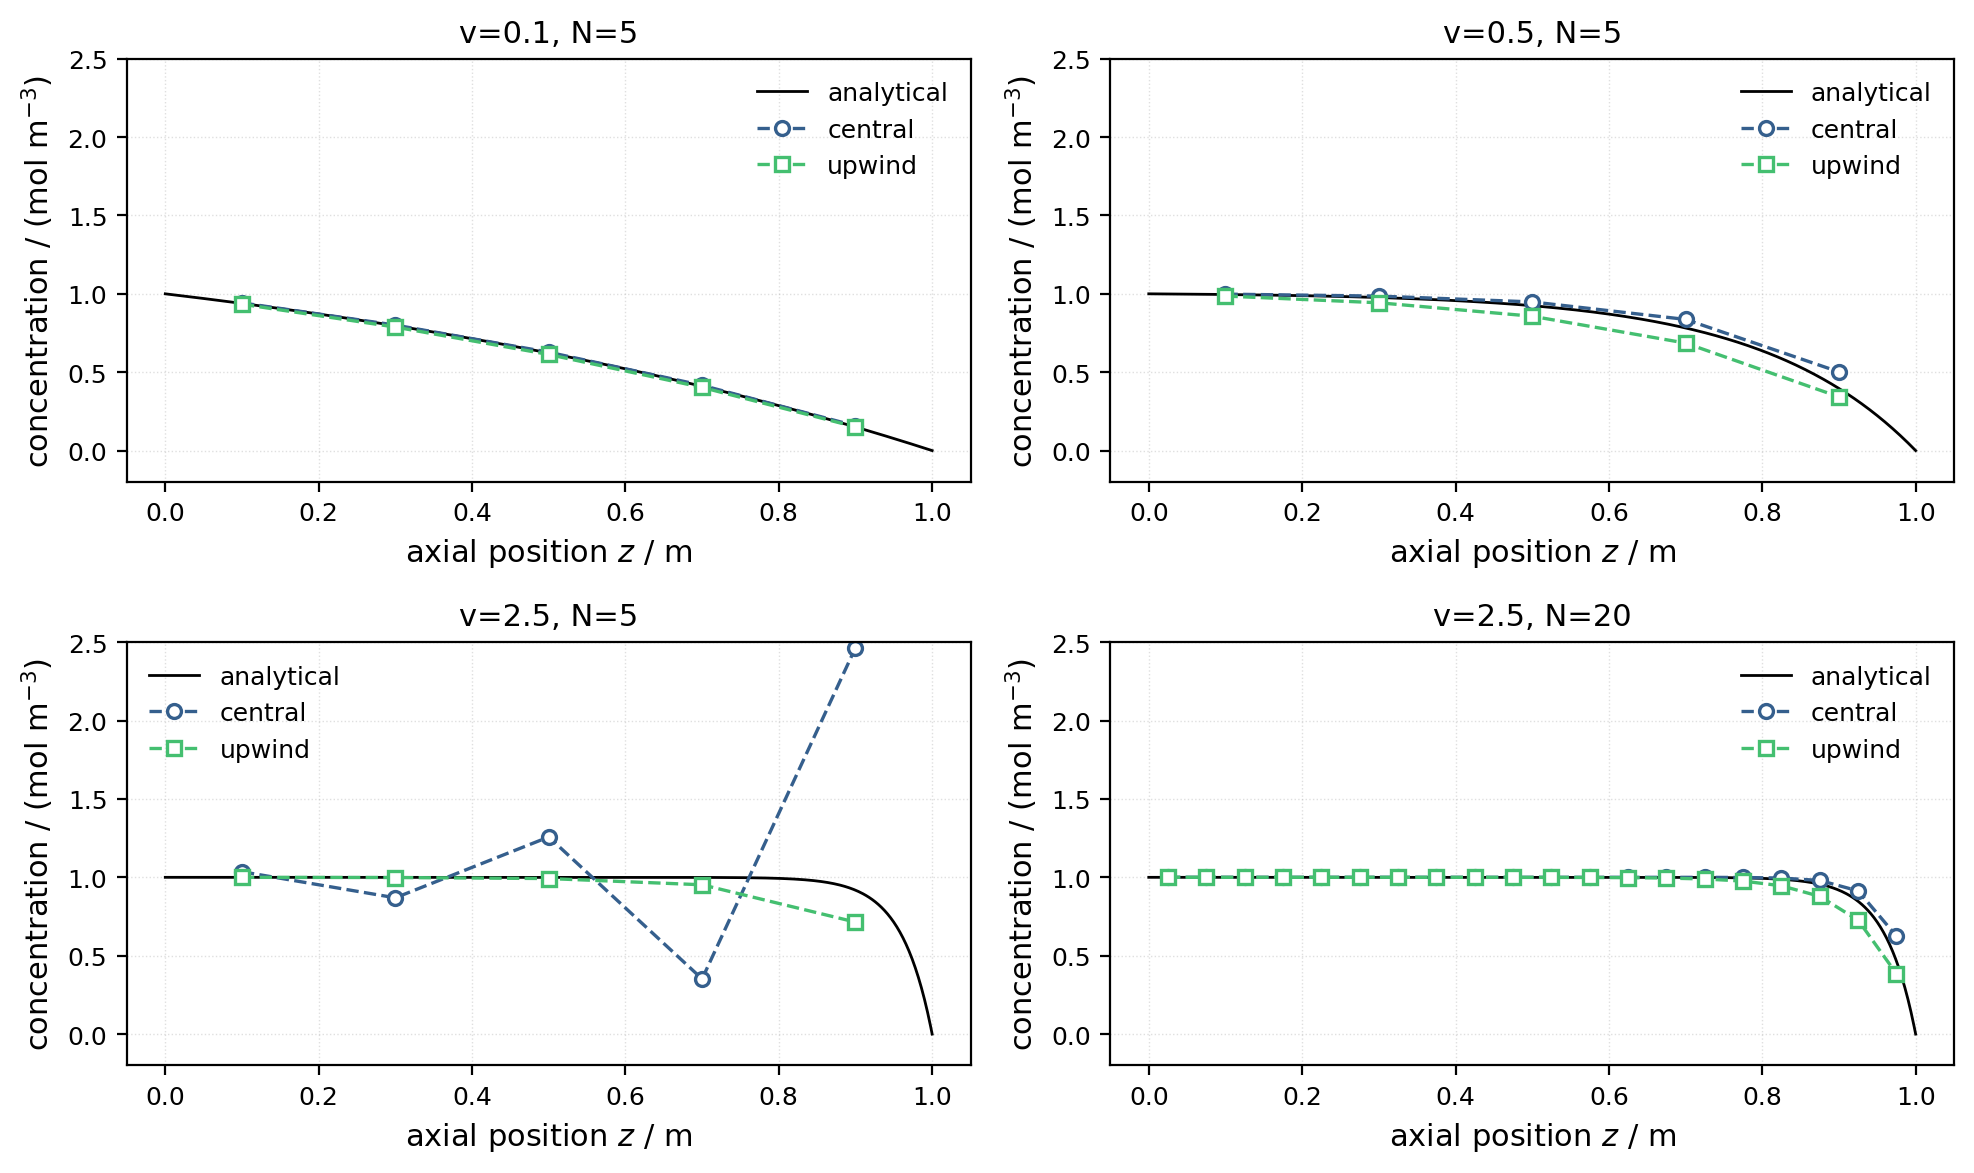
\includegraphics[width=\textwidth]{figures/fvm_comparison.png}
\caption{Central vs.\ upwind FVM schemes against the analytical solution for
steady-state convection-diffusion at four \((v, N)\) settings. As
\(\Pe_{\mathrm{cell}}\) rises, central differencing oscillates while upwind
stays monotone; refinement reduces numerical diffusion. Results from a
homework assignment given by the thesis
supervisor.}\label{fig:fvm_comparison}
\end{figure}
\FloatBarrier

\subsection{The Semi-Discrete System of ODEs}\label{ssec:semidiscrete_ode}

Substituting the upwind convective flux~\eqref{eq:upwind_flux} and the central diffusive flux~\eqref{eq:diffusive_flux_approx} into the semi-discrete \cref{eq:fvm_semidiscrete}, the governing ODE for cell~\(j\) on a uniform grid with \(u > 0\) becomes
%
\begin{equation}
  \frac{\mathrm{d}\bar{C}_{i,j}}{\mathrm{d}t}
  = -\,u\,\frac{\bar{C}_{i,j} - \bar{C}_{i,j-1}}{\Delta x}
    + \Dax\,
      \frac{\bar{C}_{i,j+1} - 2\,\bar{C}_{i,j} + \bar{C}_{i,j-1}}
           {{(\Delta x)}^{2}}
    + R_i{(\bar{\vect{C}}_j, T)}
  \label{eq:semidiscrete_full}
\end{equation}
%
for \(j = 1, 2, \ldots, N\). At the domain boundaries, the flux formulas require concentration values outside the physical domain. These are supplied by \emph{ghost cells}~\cite{LeVeque2002} --- fictitious cells placed at each end of the computational domain. At the inlet, the Dirichlet condition~\eqref{eq:dirichlet_inlet} is enforced by setting the ghost cell value to the inlet concentration, \(\bar{C}_{i,0} = \Cin\). 

The standard upwind formula at face~\(j = \tfrac{1}{2}\) then automatically produces the correct inlet flux \(F^{\mathrm{c}}_{1/2} = u\,\Cin\) without special-casing the first cell. At the outlet, the zero-gradient condition~\eqref{eq:neumann_outlet} is implemented by mirroring the last interior cell: \(\bar{C}_{i,N+1} = \bar{C}_{i,N}\). This ensures that the diffusive flux at the outlet face vanishes and convection simply carries the last cell's concentration out of the domain. 

With these ghost cell definitions, \cref{eq:semidiscrete_full} applies uniformly for all \(j = 1, \ldots, N\) without branching logic at the boundaries. Collecting all cell-averaged concentrations into a single state vector \(\vect{y}(t)\) of dimension \(N_s \times N\), where \(N_s\) is the number of species, the complete system can be written compactly as~\cite{HairerWanner1996}
%
\begin{equation}
  \frac{\mathrm{d}\vect{y}}{\mathrm{d}t} = \vect{f}(\vect{y}, t)
  \label{eq:ode_system}
\end{equation}
%
where the right-hand side \(\vect{f}\) encapsulates the convective fluxes, diffusive fluxes, and reaction source terms. For practical reactor configurations, the total number of equations \(N_s \times N\) can easily reach into the thousands. The system is stiff~\cite{HairerWanner1996} for two reasons. First, the reaction source terms span many orders of magnitude in timescale: widely varying activation energies produce both fast and slow dynamics that must be integrated simultaneously. 

Second, when \(\Dax\) is nonzero and \(\Delta x\) is small, the diffusive eigenvalues scale as \(\Dax / {(\Delta x)}^{2}\), further separating the fastest and slowest timescales. The spatial discretisation thus transforms the original PDE into a stiff ODE system --- precisely the class of problems that motivates the comparison of explicit (forward~Euler), implicit (backward~Euler with Newton iteration), and method-of-lines (BDF via ODEPACK/LSODA) integrators presented in the following chapter.

The state vector is assembled in \emph{cell-grouped ordering}: all species concentrations within each cell are stored consecutively, so that entries \((j-1)\,N_s + 1\) through \(j\,N_s\) correspond to cell~\(j\). This ordering reveals the coupling structure of the right-hand side~\(\vect{f}\). The transport terms (convection and diffusion) couple the \emph{same} species across neighbouring cells --- they link blocks that are \(N_s\) entries apart in the state vector. The reaction terms, by contrast, couple \emph{different} species within the \emph{same} cell --- they act within each block of \(N_s\) consecutive entries.

Implicit time integration methods solve a nonlinear algebraic system at every step via Newton iteration, which in turn requires evaluating and factorising the Jacobian matrix \(\vect{J} = \partial \vect{f} / \partial \vect{y}\). The cell-grouped ordering described above is directly reflected in its sparsity pattern. Because the finite volume stencil connects each cell only to its immediate neighbours, the transport terms contribute a \emph{banded} structure to~\(\vect{J}\) with bandwidth proportional to~\(N_s\). The reaction terms add dense \(N_s \times N_s\) blocks along the main diagonal, since all species within a cell are coupled through the kinetics. The resulting block-banded sparsity enables LU factorisation in \(\mathcal{O}(N_s^{2}\,N)\) operations rather than \(\mathcal{O}((N_s\,N)^{3})\) for a dense matrix~\cite{HairerWanner1996} --- a saving that makes implicit integration of the system computationally feasible.

In summary, the finite volume method has converted the original partial differential \cref{eq:species_transport} into the ODE system~\eqref{eq:ode_system} while preserving the conservation structure of the underlying physics. The telescoping property discussed in \cref{ssec:conservation_law} ensures that the stoichiometric balances of the kinetic model are maintained at the discrete level. The resulting stiff ODE system is directly suitable for the time integration methods studied in the following chapters.

% ===========================================================================
% chapters/mathematical_model.tex — Mathematical Model of the Isothermal
%                                   Tubular Reformer
% ===========================================================================

\chapter{Mathematical Model and Numerical Methods}\label{ch:reactor_model}

The previous two chapters established the building blocks. \Cref{ch:kinetic_model} fixed the lumped eight-reaction kinetic model that drives the chemistry; \cref{ch:governing_eqs} derived the convection-diffusion-reaction PDE~\eqref{eq:species_transport} and its finite-volume discretisation, ending at the per-cell semi-discrete \cref{eq:semidiscrete_full}. The present chapter pins those abstract objects to a specific physical reactor and then specifies how the resulting initial-value problem is solved numerically. \Crefrange{sec:isothermal}{sec:complete_system} fix the geometry, operating conditions, feed composition, side-stream injectors, and the few calibration choices that turn the formulation into a well-posed initial-value problem; \cref{sec:fortran,sec:solvers} then describe the implementation language and the three time-integration algorithms whose comparative performance is the subject of the next chapter.

The headline simplification carried throughout the model side of this chapter is the \emph{isothermal assumption} --- the reactor temperature is held at a single, uniform value and no enthalpy balance is solved. This decision is stated and defended in \cref{sec:isothermal}; its consequences propagate into the choice of dispersion coefficient (\cref{sec:Dax_dispersion}) and the activation-energy calibration of reaction~\eqref{eq:rxn5} retained from \cref{ssec:steam_reforming_benzene} of \cref{ch:kinetic_model}. The resulting model is best read as a benchmarking platform for the time-integration algorithms compared in the next chapter, not as a quantitative digital twin of an industrial reformer.

% ===========================================================================
% Use of Generative AI Models — unnumbered, per Saša's 2026-04-22 directive
% ===========================================================================

\section*{Use of Generative AI Models}\label{sec:ai_use}
\addcontentsline{toc}{section}{Use of Generative AI Models}

In compliance with the recommendation of the Department of Chemical Engineering and my supervisor, I declare the following regarding my use of generative artificial intelligence models in the preparation of this thesis. The single AI tool I used in the course of this work was Claude Code (Anthropic).

I used the tool for four kinds of task: review of the Fortran source code, grammar and spelling checks on the thesis text, generation of plotting scripts, and literature research. All model-level work remained with me --- including every model decision, the calibration choices documented later in this chapter, every numerical value reproduced in the thesis, the derivations of equations, and the interpretation of all results. I verified each output of the tool independently before incorporating it: I checked every literature citation against the original source via its DOI, I took every numerical value from the Fortran source of record, and my supervisor reviewed all chapters before submission. The full text of this thesis, including the literature review and the abstract, is my own work, as confirmed by the statement of authorship at the front of the document.

The AI tool was used in an editorial and exploratory capacity only; no model parameter, equation, numerical result, or interpretation reproduced in the following chapters originated from an AI tool without my independent verification.

% ===========================================================================
\section{Isothermal Assumption and Model Scope}\label{sec:isothermal}
% ===========================================================================

The temperature is held along the reactor at a single, uniform value
%
\begin{equation}
  T(x,t) \equiv T_{\mathrm{react}} = \SI{1173.15}{\kelvin}
  \quad (\approx \SI{900}{\degreeCelsius})
  \label{eq:isothermal_T}
\end{equation}
%
for every computational cell and every instant of the integration window. No enthalpy balance is solved alongside the species transport equations. Three considerations support this simplification at the present stage of the work. 

First, the primary objective of the thesis is to study the dynamic concentration evolution of a stiff reactive transport system and to benchmark candidate time-integration algorithms; isolating the chemistry from heat transfer keeps the numerical experiments interpretable. 

Second, an industrial reformer with a refractory liner and pre-heated feed approaches near-isothermal operation in its active conversion zone, so a uniform-\(T\) abstraction is a defensible first-cut model rather than an exotic choice. 

Third, decoupling chemistry from heat transfer is the standard pedagogical and prototyping starting point for tubular reactor modelling~\cite{Levenspiel1999, Fogler2006}. The isothermal assumption is not free of cost, and the chapter is honest about the price. 

Suppressing the energy balance propagates three concrete concessions through the model: one in how the rate constants are evaluated, one in how the cold reactant injectors are treated, and one in how the steam mass balance is closed. None of these are fatal in isolation, but each requires a downstream correction that this chapter has to declare openly.

(i)~I evaluate all eight Arrhenius rate constants once at the single reference temperature~\(T_{\mathrm{react}}\); the reaction source term~\(\Ri\) inherited from~\eqref{eq:species_transport} loses its \(T\)-dependence and reduces to a function of the local concentration vector alone.

(ii)~The cold side-stream injectors of oxygen and steam, which would physically enter at temperatures of order 300--500~\si{\kelvin} and locally depress the gas temperature, are introduced into a reactor that is everywhere at \SI{1173}{\kelvin}; the corresponding enthalpy sinks are ignored.

(iii)~With the steam-reforming reactions running at their full Arrhenius rate from the inlet rather than being Arrhenius-frozen by a cold inlet zone, the steam demand of the isothermal model exceeds the supply that would be reasonable for a non-isothermal reformer; this is addressed by enlarging the cell-1 \ce{H2O} injector, and the benzene steam-reforming reaction~\eqref{eq:rxn5} retains the calibrated activation energy \(E_5 = \SI{443}{\kilo\joule\per\mole}\) so that the soot-formation pathway can proceed at all.

A future extension that solves the energy balance alongside the species transport would remove both calibration choices identified above, since a cooler inlet zone naturally paces the steam-reforming reactions.

% ===========================================================================
\section{Reactor Geometry and Operating Conditions}\label{sec:geometry}
% ===========================================================================

I model the reactor as a straight cylindrical tube of length~\(L\) and constant internal diameter~\(d\), at uniform temperature~\(T_{\mathrm{react}}\) and total pressure~\(P\). I collect the geometric and operating parameters used throughout the simulations in \cref{tab:reactor_params}; they match the values hard-coded in the Fortran model that produces the simulation results of subsequent chapters.

\begin{table}[H]
\centering
\footnotesize
\caption{Reactor geometry and operating conditions; values match the Fortran model.}\label{tab:reactor_params}
\begin{tabular*}{\textwidth}{@{\extracolsep{\fill}}lll}
\toprule
Parameter & Symbol & Value \\
\midrule
Reactor length             & \(L\)            & \SI{20}{\metre} \\
Internal diameter          & \(d\)            & \SI{0.60}{\metre} \\
Cross-sectional area       & \(A = \pi d^2/4\)& \SI{0.2827}{\metre\squared} \\
Superficial gas velocity   & \(u\)            & \SI{0.516}{\metre\per\second} \\
Operating temperature      & \(T_{\mathrm{react}}\) & \SI{1173.15}{\kelvin} (\SI{900}{\degreeCelsius}) \\
Total pressure             & \(P\)            & \SI{101.325}{\kilo\pascal} \\
Number of finite volumes   & \(N\)            & 100 \\
Cell width                 & \(\Delta x = L/N\)& \SI{0.20}{\metre} \\
Axial dispersion coefficient   & \(\Dax\)     & \SI{1.0e-2}{\metre\squared\per\second}\(^{\ast}\) \\
\bottomrule
\end{tabular*}
\end{table}

The asterisk on~\(\Dax\) is unpacked in \cref{sec:Dax_dispersion}; the assumptions of \cref{sec:pfr_model} --- one-dimensional, axially symmetric, constant cross-section, approximately constant pressure --- all hold for these numbers. The mean residence time:
%
\begin{equation}
  \tau = \frac{L}{u} = \frac{20}{0.516} \approx \SI{38.8}{\second}
  \label{eq:residence_time}
\end{equation}
%
is the natural time-scale against which the integration window is calibrated. The runs reported in this chapter and the next use \(t_{\mathrm{end}} = \SI{50}{\second}\) --- slightly above one residence time --- which provides a comfortable margin past the front arrival to reach a stationary axial profile. A useful sanity check on the flow regime is the Reynolds number:
%
\begin{equation}
  \Re = \frac{u\,d}{\nu}
      = \frac{0.516 \times 0.60}{2.0\times 10^{-4}}
      \approx 1.55 \times 10^{3},
  \label{eq:reynolds_reactor}
\end{equation}
%
where \(\nu \approx \SI{2.0e-4}{\metre\squared\per\second}\) is representative for hot syngas at \SI{900}{\degreeCelsius}~\cite{Fogler2006}. The result places the flow just below the pipe-flow transition \(\Re \approx 2{,}300\), at the upper edge of the laminar regime; the implications for \(\Dax\) are unpacked in \cref{sec:Dax_dispersion}.

% ===========================================================================
\section{Feed Composition and Inlet Conditions}\label{sec:feed}
% ===========================================================================

\subsection{Species Tracked}\label{ssec:species_list}

I follow ten species in the simulation: three carbon-containing fuels (methane, benzene, an aromatic tar surrogate), the oxidant, two reforming products, the steam reactant, the soot product, and an inert diluent. They are listed in \cref{tab:species}; the index column \(i\) is the same index that appears in the state vector. I treat soot as a pseudo-gaseous species with an effective molar concentration, following the lumped approach of Jess~\cite{Jess1996}; nitrogen is purely a diluent and changes only through convective transport.

\begin{table}[H]
\centering
\footnotesize
\caption{Species tracked in the reactor model; indices follow the state-vector ordering of \cref{ssec:state_vector}.}\label{tab:species}
\begin{tabular*}{\textwidth}{@{\extracolsep{\fill}}clll}
\toprule
Index \(i\) & Species & Role in the model & Formula \\
\midrule
1  & Methane                  & Aliphatic surrogate         & \ce{CH4}   \\
2  & Benzene                  & Intermediate aromatic       & \ce{C6H6}  \\
3  & \(\alpha\)-Methylstyrene & Heavy tar surrogate         & \ce{C9H10} \\
4  & Oxygen                   & Oxidant (injected only)     & \ce{O2}    \\
5  & Carbon monoxide          & Partial-oxidation product   & \ce{CO}    \\
6  & Hydrogen                 & Product / R5 inhibitor      & \ce{H2}    \\
7  & Steam                    & Reforming agent (injected)  & \ce{H2O}   \\
8  & Carbon dioxide           & Steam-reforming product     & \ce{CO2}   \\
9  & Soot (carbon)            & Solid product               & \ce{C}     \\
10 & Nitrogen                 & Inert diluent               & \ce{N2}    \\
\bottomrule
\end{tabular*}
\end{table}

\subsection{Inlet Mole Fractions and Concentration Conversion}\label{ssec:inlet}

The full inlet composition is given in \cref{tab:inlet_composition}. At the reactor inlet, the gas is a model pyrolytic mixture dominated by the heavy aromatic surrogate and methane, with smaller contributions of hydrogen, carbon monoxide, and carbon dioxide; the oxygen and water that drive the partial-oxidation and steam-reforming chemistry are deliberately absent and enter only through the side-stream injectors. The inlet mole fractions are converted to molar concentrations via the ideal-gas law at the reactor temperature and pressure. The total molar concentration is
%
\begin{equation}
  C_{\mathrm{tot}}
  = \frac{P}{R\,T_{\mathrm{react}}}
  = \frac{\SI{101325}{\pascal}}{\SI{8.314}{\joule\per\mole\per\kelvin}\times\SI{1173.15}{\kelvin}}
  \approx \SI{10.4}{\mole\per\metre\cubed},
  \label{eq:ideal_gas_total}
\end{equation}
%
and the inlet concentration of species~\(i\) is
%
\begin{equation}
  C_{i,\mathrm{in}} = y_{i,\mathrm{in}}\,C_{\mathrm{tot}}.
  \label{eq:inlet_conc}
\end{equation}
%
\begin{table}[!t]
\centering
\footnotesize
\caption{Inlet mole fractions of the model pyrolytic gas. Unlisted species enter at zero; \ce{O2} and \ce{H2O} arrive through the side-stream injectors of \cref{sec:injectors}.}\label{tab:inlet_composition}
\begin{tabular*}{\textwidth}{@{\extracolsep{\fill}}clr}
\toprule
Index \(i\) & Species & Mole fraction \(y_{i,\mathrm{in}}\) \\
\midrule
1  & \ce{CH4}   & 0.51382 \\
3  & \ce{C9H10} & 0.39711 \\
6  & \ce{H2}    & 0.06714 \\
5  & \ce{CO}    & 0.01141 \\
8  & \ce{CO2}   & 0.01053 \\
\bottomrule
\end{tabular*}
\end{table}
%
The vector \(\Cin\) defined in this way is the concrete realisation of the inlet vector that appears in the Dirichlet condition~\eqref{eq:dirichlet_inlet} of \cref{ch:governing_eqs}, completing the specification of the feed in concentration form. The single parameter in \cref{tab:reactor_params} that still requires physical justification is the axial dispersion coefficient~\(\Dax\), whose value lies at the boundary between the laminar and transitional regimes; its derivation is the subject of the next section.
% ===========================================================================
\section{Axial Dispersion: Laminar--Turbulent Regime}\label{sec:Dax_dispersion}
% ===========================================================================

I choose \(\Dax\) carefully because the operating conditions sit at the boundary between the laminar regime, where the classical Aris-Taylor formula~\eqref{eq:aris_taylor} applies, and the transitional regime, where empirical turbulent-pipe correlations take over. Neither limit is unambiguously appropriate; the value I report in \cref{tab:reactor_params} comes from the empirical correlation, with its limits and assumptions stated openly. A laminar Aris-Taylor estimate~\cite{Taylor1953, Aris1956}, with molecular diffusivity \(D_{AB} \approx \SI{2e-4}{\metre\squared\per\second}\) for light gases at \SI{900}{\degreeCelsius}~\cite{Fogler2006} and the geometry of \cref{tab:reactor_params} (\(u = \SI{0.516}{\metre\per\second}\), tube radius \(R = d/2 = \SI{0.30}{\metre}\)), gives
%
\begin{equation*}
  \Dax^{\mathrm{Aris-Taylor}}
  = D_{AB} + \frac{u^2 R^2}{48\,D_{AB}}
  \approx 2\times 10^{-4} + \frac{(0.516)^2 (0.30)^2}{48\times 2\times 10^{-4}}
  \approx \SI{2.5}{\metre\squared\per\second}.
\end{equation*}
%
This estimate rests on the assumption of a fully developed laminar parabolic profile, which is violated for the present reactor on three counts: the side-injection ports introduce strong cross-sectional concentration gradients near each injector cell; the axial density variation produced by reactions~\eqref{eq:rxn1}--\eqref{eq:rxn8} (mean molar mass falling from \(\overline{M}\approx\SI{56}{\gram\per\mol}\) at the inlet to \(\overline{M}\approx\SI{30}{\gram\per\mol}\) once steam reforming has converted the heavy hydrocarbons) breaks the constant-property assumption; and the Reynolds number of \cref{eq:reynolds_reactor} sits at the upper edge of the laminar band, so any of these perturbations can plausibly trip the flow into transitional behaviour. The Aris-Taylor formula is therefore an upper bound, not a defensible point estimate. A more appropriate framework for this regime is the empirical correlation of axial dispersion in turbulent pipe flow reported by Levenspiel~\cite{Levenspiel1999}. He reports the dimensionless Bodenstein number \(\mathrm{Pe}_d = u\,d/\Dax\) in the band \(1\)--\(10\) for \(\Re\) between roughly~\(2{,}000\) and~\(10{,}000\), with the lower edge of that band corresponding to flows near the laminar transition. The present operating point at \(\Re \approx 1{,}550\) lies just below the calibration range of this correlation: a direct extrapolation toward lower \(\Re\) would push \(\mathrm{Pe}_d\) further down (i.e.\ \(\Dax\) further up), in the same direction as the laminar Aris-Taylor estimate above. I therefore depart from a strict application of the correlation and adopt \(\mathrm{Pe}_d \approx 30\), several times below the \(\Dax\) the correlation would predict at fully developed turbulent conditions, giving
%
\begin{equation*}
  \Dax = \frac{u\,d}{\mathrm{Pe}_d}
       = \frac{0.516 \times 0.60}{30}
       \approx \SI{1.0e-2}{\metre\squared\per\second},
\end{equation*}
%
which is the value listed in \cref{tab:reactor_params}. The remaining sanity checks on this choice are the global P\'eclet number for the full reactor length
%
\begin{equation}
  \Pe = \frac{u\,L}{\Dax}
      = \frac{0.516 \times 20}{10^{-2}}
      \approx 1{,}032,
  \label{eq:pe_reactor}
\end{equation}
%
which keeps the reactor strongly convection-dominated, and the cell P\'eclet number on the uniform grid of \cref{tab:reactor_params}
%
\begin{equation}
  \Pe_{\mathrm{cell}}
  = \frac{u\,\Delta x}{\Dax}
  = \frac{0.516 \times 0.20}{10^{-2}}
  \approx 10,
  \label{eq:pe_cell}
\end{equation}
%
which is well above the central-differencing stability threshold of~2. The first-order upwind scheme of \cref{eq:upwind} is therefore the appropriate choice for the convective flux. A complementary characteristic length is the Taylor smearing distance accumulated over the residence time of \cref{eq:residence_time},
%
\begin{equation*}
  \sigma = \sqrt{2\Dax\,\tau} \approx \SI{0.88}{\metre},
\end{equation*}
%
about four cells, which is small enough to preserve the cell-1 front-loaded steam profile, and large enough that the dispersion contribution to the system Jacobian is non-trivial and improves the conditioning of the implicit time-integration solvers compared with the pure-PFR limit \(\Dax \to 0\). Substituting the Aris-Taylor value \(\Dax \approx \SI{2.5}{\metre\squared\per\second}\) directly into the isothermal model was confirmed empirically to break the chemistry: at \(\Pe \approx 4\) the reactor enters the diffusion-dominated regime, the cell-1 \ce{H2O} boost smears across the whole reactor within one residence time, and the steam-reforming reactions shut off under the \(\max(\bar{C}_{i,j}, 0)\) clamp. The isothermal assumption combined with fully laminar dispersion has no operating point at which the chemistry both runs to completion and conserves steam; the proper resolution is the energy-balance extension of \cref{sec:isothermal}.

% ===========================================================================
\section{Side-Injection Model for Oxygen and Steam}\label{sec:injectors}
% ===========================================================================

\subsection{Physical Motivation}\label{ssec:injector_motivation}

The pyrolytic gas entering the reactor is dry: oxygen and water are absent from the inlet stream listed in \cref{tab:inlet_composition}. Both reactants are introduced through nine discrete side-stream injectors, but with rather different axial distributions. 

Oxygen is staged along the length of the reactor: it sustains the partial-oxidation reactions~\eqref{eq:rxn1}--\eqref{eq:rxn3} past the initial inlet zone, where they would otherwise be quenched by oxygen depletion, and the staged supply mimics the feed design used in industrial reformers to control hot-spot formation and to extend the active reaction zone. Steam, by contrast, is overwhelmingly concentrated at the inlet (cell~1), with the eight downstream injectors providing only top-up amounts. 

This front-loaded layout closes the isothermal steam mass balance --- the third concession identified in \cref{sec:isothermal} --- and is reflected in the cell-1 \ce{H2O} flow rate of \cref{tab:injectors}. Steam itself drives the reforming reactions~\eqref{eq:rxn4}--\eqref{eq:rxn6} and the soot gasification of \cref{eq:rxn8}.

\subsection{Logical-Switch Source Term}\label{ssec:logical_switch}

In the finite-volume framework of \cref{ch:governing_eqs}, each injector is modelled as a point source localised to a single computational cell. Following the design pattern proposed by the supervisor, every cell formally carries an injector slot for every species, but the slot contributes only when a logical switch is on. 

Consider \(K\) injectors, with the \(k\)-th delivering molar flow \(\dot{n}_{i,\mathrm{inj}}^{(k)}\) [\si{\mole\per\second}] of species~\(i\) into cell \(j_{\mathrm{inj}}^{(k)}\). Distributing each injection uniformly over its cell volume \(V_{\mathrm{cell}} = A\,\Delta x\) and summing over all injectors gives the volumetric source \(S_{\mathrm{i,j}}\) where the Kronecker delta selects only the host cell of each injector. The result has units of \si{\mole\per\metre\cubed\per\second}, matching the reaction source~\(R_i\) inherited from~\eqref{eq:species_transport}.
%
\begin{equation}
  S_{i,j}
  = \sum_{k=1}^{K} \frac{\dot{n}_{i,\mathrm{inj}}^{(k)}}{A\,\Delta x}\,
    \delta_{j,\,j_{\mathrm{inj}}^{(k)}},
  \label{eq:injection_total}
\end{equation}
%


\subsection{Injector Locations and Flow Rates}\label{ssec:injector_table}

\begin{figure}[H]
\centering
\resizebox{\textwidth}{!}{%
\begin{tikzpicture}[>=stealth, thick, every node/.style={font=\small}]
  % Drawing scale: 1 m of reactor -> \Lscale cm of drawing width
  \def\Lscale{0.65}
  % Reactor tube
  \draw[thick, fill=gray!10]
    (0, 0) rectangle (\Lscale*20, 1.0);
  % Inlet feed arrow
  \draw[->, very thick, blue!70!black]
    (-1.4, 0.5) -- (-0.05, 0.5)
    node[midway, above, font=\footnotesize] {feed};
  % Outlet arrow
  \draw[->, very thick, blue!70!black]
    (\Lscale*20+0.05, 0.5) -- (\Lscale*20+1.4, 0.5)
    node[midway, above, font=\footnotesize] {outlet};
  % Injector arrows with rotated labels to avoid collision in the dense inlet zone
  \foreach \pos/\k in {0/1, 0.5/2, 1/3, 2/4, 3/5, 5/6, 8/7, 13/8, 19/9} {
    \draw[->, red!70!black, thick]
      (\Lscale*\pos, -0.9) -- (\Lscale*\pos, 0);
    \node[font=\scriptsize, red!50!black, rotate=60, anchor=north east]
      at (\Lscale*\pos, -0.95) {\(k=\k\)};
  }
  % Injection species label centered below
  \node[font=\footnotesize, red!50!black]
    at (\Lscale*10, -2.4) {\ce{O2} \;+\; \ce{H2O} side injectors};
  % Length annotation
  \draw[decorate, decoration={brace, mirror, amplitude=4pt}]
    (\Lscale*20, 1.15) -- (0, 1.15)
    node[midway, above=4pt, font=\footnotesize] {\(L = \SI{20}{\metre}\)};
  % Diameter annotation inside reactor between injectors 4 and 5 (per Saša 2026-05-17)
  \draw[<->, gray!60!black, thin]
    (\Lscale*2.5, 0.05) -- (\Lscale*2.5, 0.95)
    node[pos=0.5, right=2pt, font=\scriptsize, gray!60!black] {\(d\)};
\end{tikzpicture}%
}
\caption{Schematic of the isothermal tubular reformer (not to scale). Nine side-stream injectors, indexed \(k = 1, \ldots, 9\), introduce oxygen and steam at axial positions given in \cref{tab:injectors}.}%
\label{fig:reactor_schematic}
\end{figure}

Nine injection ports are distributed along the reactor axis. The cell indices are obtained by mapping each axial position onto the uniform grid of cell centres \(x_j = (j - \tfrac{1}{2})\,\Delta x\) with \(\Delta x = \SI{0.20}{\metre}\), giving the index sequence \(j_{\mathrm{inj}}^{(k)} \in \{1, 3, 5, 10, 15, 25, 40, 65, 95\}\). The first three ports cluster within the first metre of the reactor: they sustain partial oxidation through the inlet zone (oxygen) and pre-load the steam reservoir for the steam-reforming reactions that begin immediately at \(T_{\mathrm{react}}\) (water). The downstream ports thin out toward the outlet, reflecting the diminishing demand once the aromatic load has been largely converted. \Cref{fig:reactor_schematic} shows the layout schematically; the numerical values of all nine injectors are listed in \cref{tab:injectors}.

\begin{table}[H]
\centering
\footnotesize
\caption{Side-stream injector positions and molar flow rates. Cell-1 water is enlarged to \SI{6.0}{\mole\per\second} (reference \SI{0.166}{\mole\per\second}) to close the isothermal steam balance.}\label{tab:injectors}
\begin{tabular*}{\textwidth}{@{\extracolsep{\fill}}cccrr}
\toprule
\(k\) & Position [m] & Cell \(j_{\mathrm{inj}}^{(k)}\) &
  \(\dot{n}_{\mathrm{O_2}}^{(k)}\) [\si{\mole\per\second}] &
  \(\dot{n}_{\mathrm{H_2O}}^{(k)}\) [\si{\mole\per\second}] \\
\midrule
1 & 0.0  & 1  & 0.205 & \textbf{6.000} \\
2 & 0.5  & 3  & 0.240 & 0.590 \\
3 & 1.0  & 5  & 0.200 & 0.560 \\
4 & 2.0  & 10 & 0.210 & 0.430 \\
5 & 3.0  & 15 & 0.170 & 0.390 \\
6 & 5.0  & 25 & 0.180 & 0.240 \\
7 & 8.0  & 40 & 0.160 & 0.060 \\
8 & 13.0 & 65 & 0.150 & 0.010 \\
9 & 19.0 & 95 & 0.160 & 1\,\(\times 10^{-6}\) \\
\midrule
  & Total & & 1.675 & 8.280 \\
\bottomrule
\end{tabular*}
\end{table}
\FloatBarrier

% ===========================================================================
\needspace{8\baselineskip}% keep \section{} from orphaning above its first \subsection
\section{Complete Semi-Discrete ODE System}\label{sec:complete_system}
% ===========================================================================

\subsection{Governing ODE per Cell}\label{ssec:per_cell_ode}

Specialising the per-cell semi-discrete \cref{eq:semidiscrete_full} of \cref{ch:governing_eqs} by adding the injection source term~\eqref{eq:injection_total}, the governing ordinary differential equation for species~\(i\) in cell~\(j\) becomes
%
\begin{equation}
  \frac{\mathrm{d}\bar{C}_{i,j}}{\mathrm{d}t}
  = \underbrace{-\,u\,\frac{\bar{C}_{i,j} - \bar{C}_{i,j-1}}{\Delta x}}_{\text{convection}}
  \;+\; \underbrace{\Dax\,\frac{\bar{C}_{i,j+1} - 2\,\bar{C}_{i,j} + \bar{C}_{i,j-1}}{(\Delta x)^{2}}}_{\text{diffusion}}
  \;+\; \underbrace{R_i(\bar{\vect{C}}_j)}_{\text{reaction}}
  \;+\; \underbrace{S_{i,j}}_{\text{injection}},
  \label{eq:full_per_cell}
\end{equation}
%
for \(j = 1, \ldots, N\) and \(i = 1, \ldots, N_s\). The reaction term~\(R_i(\bar{\vect{C}}_j)\) carries no explicit temperature dependence here, as a direct consequence of the isothermal assumption~\eqref{eq:isothermal_T}: the rate constants are evaluated once at \(T_{\mathrm{react}}\) using the Arrhenius parameters of \cref{ch:kinetic_model}. The boundary treatment is inherited unchanged from \cref{ssec:semidiscrete_ode}: a Dirichlet ghost cell \(\bar{C}_{i,0} = C_{i,\mathrm{in}}\) at the inlet and a zero-gradient ghost cell \(\bar{C}_{i,N+1} = \bar{C}_{i,N}\) at the outlet, so \cref{eq:full_per_cell} applies uniformly across all cells.

\subsection{State Vector and System Dimension}\label{ssec:state_vector}

All cell-averaged concentrations are stacked into a single state vector \(\vect{y}(t)\) of dimension \(N_s \times N\). The Fortran model uses a \emph{cell-grouped, species-fastest} ordering, in which the species index \(i\) varies fastest within each cell block:
%
\begin{equation}
  y_{(j-1)\,N_s + i}(t) = \bar{C}_{i,j}(t),
  \qquad i = 1, \ldots, N_s,
  \;\; j = 1, \ldots, N.
  \label{eq:state_vector_ordering}
\end{equation}
%
With \(N_s = 10\) species and \(N = 100\) cells, the state vector contains \(1{,}000\) unknowns. The cell-grouped ordering keeps the data accessed by the finite-volume stencil contiguous in memory --- evaluating the right-hand side of \cref{eq:full_per_cell} for cell~\(j\) touches three consecutive blocks of ten doubles --- which is the natural choice for the stencil-driven RHS assembly of the model.

Collecting the per-cell equations~\eqref{eq:full_per_cell} into vector form gives the compact system
%
\begin{equation}
  \frac{\mathrm{d}\vect{y}}{\mathrm{d}t}
  = \vect{f}_{\mathrm{conv}}(\vect{y})
  + \vect{f}_{\mathrm{diff}}(\vect{y})
  + \vect{f}_{\mathrm{rxn}}(\vect{y})
  + \vect{s},
  \label{eq:ode_split}
\end{equation}
%
where the four terms collect the convective, diffusive, reactive, and injection contributions respectively. The injection vector~\(\vect{s}\) is constant in time and depends on neither~\(\vect{y}\) nor~\(t\), so it does not contribute to the Jacobian \(\vect{J} = \partial \vect{f}/\partial \vect{y}\); the block-banded sparsity pattern of \(\vect{J}\) discussed in \cref{ssec:semidiscrete_ode} is therefore preserved unchanged.

The initial condition adopted in this work is a vacuum,
%
\begin{equation}
  \bar{C}_{i,j}(0) = 0
  \quad\text{for all}\quad i = 1, \ldots, N_s,\; j = 1, \ldots, N.
  \label{eq:ic_vacuum}
\end{equation}
%
This represents an empty reactor at \(t = 0\), when feed and side-stream injectors are switched on. The vacuum start avoids an artefact of the uniform-feed alternative \(\bar{C}_{i,j}(0) = C_{i,\mathrm{in}}\), which would place \ce{C9H10} at its inlet value in every cell and trigger reaction~\eqref{eq:rxn6} on non-existent steam before the cell-1 wavefront arrives. A startup transient of roughly \(\tau\) follows, after which the steady state is established; alternative initial conditions (uniform feed, \ce{N2}-purged, steam-purged) give the same steady state.

% ===========================================================================
\section{Choice of Implementation Language}\label{sec:fortran}
% ===========================================================================

The simulation reported in this thesis is implemented in Fortran. The choice was made on my supervisor's recommendation, motivated by Fortran's well-documented performance advantage on arithmetic-heavy numerical workloads: benchmarks consistently place ahead-of-time compiled languages in the top tier and interpreted alternatives such as Python one to two orders of magnitude behind~\cite{Pereira2017}. This advantage matters specifically for the present work, where the same right-hand-side function is evaluated under three different time-integration algorithms; any per-call overhead introduced by a slower runtime would pollute the wall-clock measurements and make the comparison reflect the language environment rather than the algorithms themselves. Fortran (\emph{Formula Translation}) was developed at IBM by John Backus and his team and first published in 1957~\cite{Backus1957} with the explicit objective of producing a high-level language whose compiler would emit machine code competitive with hand-written assembly for scientific calculations; almost seven decades of refinement have followed~\cite{MetcalfReidCohen2018}, all aimed at tight loops over arrays of numbers. The performance follows from two design choices: ahead-of-time compilation, which translates the source into the exact CPU instructions before the program runs --- where Python and MATLAB translate each line on the fly, roughly the difference between reading a book already translated and listening to a live interpreter at a conference; and automatic vectorisation, where the compiler safely emits CPU instructions that perform several arithmetic operations per clock cycle on ordinary loops, while higher-level languages reach this level only through compiled libraries, with per-call overhead that dominates on small per-cell arrays. The same algorithm therefore completes in seconds where equivalent Python or MATLAB code would take minutes, and the wall-clock differences reported in the next chapter reflect the algorithms themselves, not the language.

% ===========================================================================
\section{Time-Integration Algorithms}\label{sec:solvers}
% ===========================================================================

Three time-integration algorithms are implemented and benchmarked, each representing one canonical strategy: forward Euler, an explicit fixed-step method; backward Euler with a banded Newton iteration, an implicit fixed-step method; and the variable-step, variable-order backward differentiation formula (BDF) family in DLSODE~\cite{Hindmarsh1983}, an adaptive method-of-lines solver. All three operate on the same right-hand side~\(\vect{f}\) of \cref{eq:ode_split} and differ only in their internal step structure.

\subsection{Forward Euler}\label{ssec:forward_euler}

The forward Euler scheme advances the state by the explicit update
\begin{equation}
  \vect{y}_{n+1} = \vect{y}_n + \Delta t\,\vect{f}(\vect{y}_n),
  \label{eq:fwd_euler}
\end{equation}
costing one right-hand-side evaluation per step and yielding first-order accuracy in time. The method is only conditionally stable; for the convection-diffusion-reaction discretisation of \cref{ch:governing_eqs} the dominant restriction is the Courant--Friedrichs--Lewy (CFL) condition
\begin{equation}
  \Delta t \;<\; \frac{\Delta x}{u},
  \label{eq:cfl}
\end{equation}
which evaluates to \(\Delta t < \SI{0.39}{\second}\) at the standard configuration of \cref{tab:reactor_params}. The reactive source term~\(R_i\) imposes a secondary stability bound through the largest Arrhenius rate constant, but at \(T_{\mathrm{react}} = \SI{1173}{\kelvin}\) the chemical timescales remain well above the convective limit and the CFL constraint is the binding one.

The default integration step adopted here is \(\Delta t = \SI{1}{\milli\second}\), three orders of magnitude below the CFL bound. A divergence guard aborts the integration whenever any state component exceeds \(10^{15}\) in magnitude or becomes non-finite; the safety net is exercised in the next chapter, where pushing \(\Delta t\) past the CFL limit produces a numerical blow-up.

\subsection{Backward Euler with Banded Newton}\label{ssec:backward_euler}

The implicit counterpart of \cref{eq:fwd_euler} is the backward Euler step
\begin{equation}
  \vect{y}_{n+1} = \vect{y}_n + \Delta t\,\vect{f}(\vect{y}_{n+1}),
  \label{eq:bwd_euler}
\end{equation}
in which the right-hand side is evaluated at the unknown end-of-step state. The method is unconditionally A-stable for any step size~\(\Delta t > 0\), removing the CFL restriction at the price of the necessity of solving a generally nonlinear algebraic system at every integration step.

Solving \cref{eq:bwd_euler} for \(\vect{y}_{n+1}\) is cast as the residual root-finding problem
\begin{equation}
  \vect{g}(\vect{y}_{n+1}) \;=\; \vect{y}_{n+1} - \vect{y}_n - \Delta t\,\vect{f}(\vect{y}_{n+1}) \;=\; \vect{0},
  \label{eq:newton_residual}
\end{equation}
solved by Newton iteration. The Newton update reads
\begin{equation*}
  \vect{J}\,\bm{\delta} = -\vect{g}(\vect{y}^{(k)}), \qquad \vect{y}^{(k+1)} = \vect{y}^{(k)} + \bm{\delta},
\end{equation*}
with iteration Jacobian
\begin{equation*}
  \vect{J} \;=\; \frac{\partial \vect{g}}{\partial \vect{y}} \;=\; \vect{I} - \Delta t\,\frac{\partial \vect{f}}{\partial \vect{y}}
\end{equation*}
constructed by finite differences. The matrix \(\partial\vect{f}/\partial\vect{y}\) inherits the block-banded sparsity pattern of \cref{ssec:state_vector}, with lower and upper half-bandwidths \(\mathrm{ML} = \mathrm{MU} = N_s = 10\).

Curtis--Powell--Reid colouring~\cite{Curtis1974} exploits this band structure: because each column of the Jacobian affects only a narrow strip of rows, columns at sufficient distance from each other can be perturbed simultaneously without their effects overlapping. The number of right-hand-side evaluations needed to assemble the full Jacobian is therefore \(\mathrm{ML} + \mathrm{MU} + 1 = 21\) rather than \(N_{\mathrm{eqs}} = 1{,}000\). The factorisation is performed by the LINPACK banded LU routines bundled with ODEPACK; for the present bandwidth, the per-factor cost drops from \(\mathcal{O}(N_{\mathrm{eqs}}^{3})\) for a dense system to \(\mathcal{O}(\mathrm{ML}\cdot\mathrm{MU}\cdot N_{\mathrm{eqs}})\), a factor of approximately \(2{,}300\) on the standard grid.

At each integration step the Newton iteration is initialised at \(\vect{y}^{(0)} = \vect{y}_n\); the Jacobian is built and factored once at this initial guess, and the factorisation is reused for subsequent corrections. Convergence is declared when \(\lVert\bm{\delta}\rVert_\infty\) falls below a relative tolerance of \(10^{-6}\). If two successive corrections fail to halve in magnitude the Jacobian is rebuilt at the current iterate, on the assumption that the cached factorisation no longer represents the local landscape; the iteration is capped at twenty Newton steps to guarantee a graceful abort on non-convergent inputs. At the default step size \(\Delta t = \SI{10}{\milli\second}\), Newton converges in two to three steps over most of the trajectory, with one Jacobian build per integration step in the smooth regime and an occasional rebuild during the inlet startup transient.

\subsection{Method of Lines via DLSODE}\label{ssec:lsoda}

In contrast to the fully discrete schemes of \cref{ssec:forward_euler,ssec:backward_euler}, where the time variable is collapsed onto a fixed-step recurrence at the user's prescription, the method of lines treats the spatial discretisation and the time integration as separate concerns: the semi-discrete ODE system of \cref{eq:ode_split} is handed to a general-purpose ODE solver that selects its own internal time discretisation adaptively. The integrator used in this work is DLSODE from the ODEPACK library~\cite{Hindmarsh1983}, a stiff ODE solver based on the backward differentiation formulae (BDF) of orders one through five --- linear multistep schemes that combine several past states in the implicit relation
\begin{equation*}
  \sum_{j=0}^{k}\alpha_j\,\vect{y}_{n+1-j} = \Delta t\,\beta_0\,\vect{f}(\vect{y}_{n+1}),
\end{equation*}
of which backward Euler (\(k = 1\)) is the simplest case. As in \cref{ssec:backward_euler}, the implicit step is solved by a Newton iteration, but DLSODE caches and reuses the factored Jacobian across multiple steps until convergence quality degrades, amortising the dominant cost of stiff integration. DLSODE is configured here with method flag \(\mathrm{mf} = 25\), which selects the BDF family with an internally generated banded finite-difference Jacobian whose half-bandwidths match the FVM stencil, \(\mathrm{ML} = \mathrm{MU} = N_s\). Local error tolerances are set to \(10^{-5}\) relative and \(10^{-9}\) absolute.

Two adaptive mechanisms distinguish DLSODE from the fixed-step backward Euler scheme of \cref{ssec:backward_euler}. First, the step size~\(\Delta t\) is selected at every internal step from a local truncation error estimate based on the predictor--corrector difference: it grows where the solution is smooth and contracts automatically as the inlet transient injects sharp fronts into the reactor. Second, the BDF order~\(k\) varies between one and five under the same work-per-accuracy heuristic, with higher~\(k\) yielding smaller truncation error per step at the price of more state history. 

On the present problem the order typically escalates to BDF-3 or BDF-4 once the inlet transient has decayed, and the total internal step count over the \SI{50}{\second} integration window ranges from approximately one hundred at the coarsest grid to over one thousand at the finest. These adaptive mechanisms remove the need for hand-tuned step sizing and provide a documented level of local accuracy; they are also the source of the per-step overhead that the comparison in the next chapter quantifies.


% ===========================================================================
% chapters/results_and_discussions.tex — Results and Discussion
% ===========================================================================

\chapter{Results and Discussion}\label{ch:results}

This chapter is divided in two halves. The first reports the engineering output of the isothermal model: the steady-state concentration profiles of all ten species along the reactor at the design operating point, together with short parametric studies over three independent process levers --- reactor temperature, feed velocity, and side-injection mass flow. The second half benchmarks the three time-integration algorithms on the same model: wall-clock time on the real eight-reaction problem, max-norm relative error on a simplified single-reaction reactor with an analytical reference, and an explicit-vs-implicit Euler comparison at a fixed grid. The two halves are combined into a single solver recommendation at the end. The eight reactions of the kinetic model from \cref{ch:kinetic_model} are recapped in \cref{tab:reactions_recap} and referenced as R1--R8 throughout this chapter.

\begin{table}[H]
\centering
\footnotesize
\caption{The eight global reactions of the adopted kinetic scheme.}\label{tab:reactions_recap}
\begin{tabular*}{\textwidth}{@{\extracolsep{\fill}} l l l}
\toprule
 & Reaction & Process \\
\midrule
R1 & \ce{CH4 + \frac{1}{2} O2 -> CO + 2 H2}                                   & methane partial oxidation \\
R2 & \ce{C6H6 + 3 O2 -> 6 CO + 3 H2}                                          & benzene partial oxidation \\
R3 & \ce{C9H10 + \frac{9}{2} O2 -> 9 CO + 5 H2}                               & \(\alpha\)-methylstyrene partial oxidation \\
R4 & \ce{CH4 + H2O -> CO + 3 H2}                                              & methane steam reforming \\
R5 & \ce{C6H6 + 2 H2O -> 2 CO + \frac{5}{2} CH4 + \frac{3}{2} C}              & benzene steam reforming \\
R6 & \ce{C9H10 + 11.5 H2O -> 6.5 CO + 2.5 CO2 + 16.5 H2}                      & \(\alpha\)-methylstyrene steam reforming \\
R7 & \ce{C9H10 + 4 H2 -> 3 CH4 + C6H6}                                        & hydrodealkylation \\
R8 & \ce{C + H2O -> CO + H2}                                                  & soot gasification \\
\bottomrule
\end{tabular*}
\end{table}

% ===========================================================================
\section{Standardised Test Conditions}\label{sec:test_conditions}
% ===========================================================================

All runs reported in this chapter were executed on a single workstation (AMD Ryzen~7 5800X3D, 8 cores / 16 threads, \SI{32}{\gibi\byte} memory, Ubuntu~24.04~LTS) using \texttt{gfortran 13.3.0} with the flags \texttt{-O2 -Wall -Wextra -fcheck=all -std=f2018}. Standardised here does not mean that the solvers share a step size or a tolerance --- there is no single setting that means the same thing across an explicit fixed-step method, an implicit fixed-step method, and an adaptive method-of-lines solver. It means that each solver is used as it is meant to be used, and the comparison reflects what each is designed to do rather than an imposed common configuration. The per-solver defaults that anchor the three numerical tests below are listed in \cref{tab:test_conditions}; the engineering profiles are all integrated with DLSODE at its default tolerances, since the engineering content is independent of the time integrator.

\begin{table}[H]
\centering
\footnotesize
\caption{Standardised test conditions; each solver at its default configuration.}\label{tab:test_conditions}
\begin{tabular*}{\textwidth}{@{\extracolsep{\fill}}lll}
\toprule
Solver & Type & Defaults \\
\midrule
Forward Euler  & explicit fixed-step       & \(\Delta t = \SI{1}{\milli\second}\) \\
Backward Euler & implicit fixed-step       & \(\Delta t = \SI{10}{\milli\second}\); Newton tolerance \(10^{-6}\) \\
DLSODE         & adaptive method-of-lines  & \(\mathrm{mf} = 25\)\footnotemark; \(\mathrm{rtol} = 10^{-5}\), \(\mathrm{atol} = 10^{-9}\) \\
\bottomrule
\end{tabular*}
\end{table}
\footnotetext{DLSODE's method flag; \(\mathrm{mf}=25\) selects the variable-order BDF integrator with an internally-generated banded Jacobian.}

% ===========================================================================
\section{Concentration Profiles Along the Reactor}\label{sec:profiles}
% ===========================================================================

The reactor design point sits inside a multidimensional operating envelope, and three of its dimensions are tunable in principle from a control room: reactor temperature, feed velocity, and the total mass flow delivered by the side injectors. This section asks what each of those three knobs does to the steady-state product distribution. The base case fixes all three at their nominal design values and establishes the reaction-zone structure the parametric variations will then perturb; each of the following three subsections varies one knob while holding the other two fixed at the design value (\(T = \SI{1173.15}{\kelvin}\), \(u = \SI{0.516}{\metre\per\second}\), and the calibrated per-injector mass flow rates). By the end, only one of the three knobs will turn out to have a non-monotonic optimum within the tested range --- and that one is therefore the most directly useful for any future parametric optimisation of the design. All four figures share a single grid resolution (\(N_\mathrm{cells} = 200\)) and the DLSODE adaptive integrator at the defaults of \cref{tab:test_conditions}.

\subsection{Design operating point}\label{ssec:profiles_base}

\begin{figure}[H]
\centering
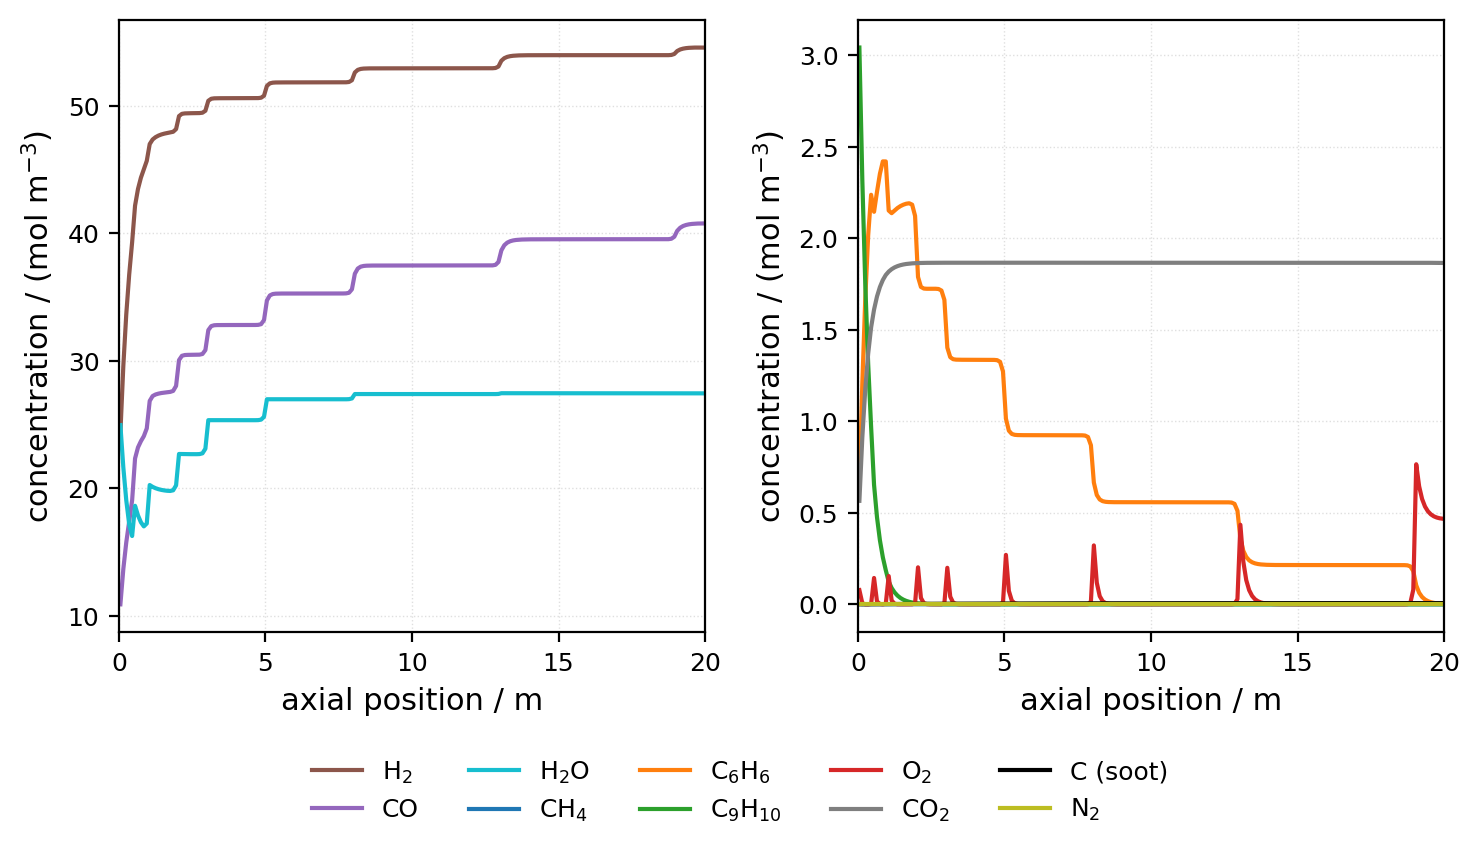
\includegraphics[width=0.95\textwidth]{figures/profiles_base.png}
\caption{Steady-state axial concentration profiles of all ten species at the design operating point (\(T = \SI{1173.15}{\kelvin}\), \(u = \SI{0.516}{\metre\per\second}\)). The two panels separate the major species (upper) from the trace species (lower) so that the two concentration scales remain legible. Methane is consumed in the first cell and does not appear in the legend.}\label{fig:profiles_base}
\end{figure}

The base case asks the simplest possible question: what does the reactor produce when all three control knobs are at their nominal design values? \Cref{fig:profiles_base} provides the answer. The two panels separate the major species (left, \SI{10}{}--\SI{55}{\mole\per\metre\cubed}) from the minor and trace species (right). Three reaction zones are visible. Within the first half-metre the pyrolytic tar precursor C\(_9\)H\(_{10}\) and the inlet methane are consumed essentially completely by partial oxidation against the dense O\(_2\) supply at the first two injectors (R1 and R3); CH\(_4\) is below its numerical floor from cell~1 onward and therefore does not appear in the legend. The two oxidation reactions emit CO, H\(_2\), and a secondary tar intermediate C\(_6\)H\(_6\), whose concentration peaks at \(\approx\SI{2.4}{\mole\per\metre\cubed}\) just downstream of the inlet bank.

Between \(x \approx \SI{0.5}{\metre}\) and \(x \approx \SI{13}{\metre}\) the reactor is in a steam-reforming regime: each O\(_2\) injector (the sharp red spikes on the right panel) is paired with an H\(_2\)O injector, and together they drive benzene oxidation, methane steam reforming, and benzene steam reforming. The combined effect is visible on every species profile as a staircase aligned with the injector positions; the C\(_6\)H\(_6\) curve in particular loses roughly half its remaining concentration at each step. From \(x \approx \SI{13}{\metre}\) to the outlet, the principal reforming and partial-oxidation reactions have run to completion: the inlet methane and \(\alpha\)-methylstyrene were consumed within the first half-metre, the benzene intermediate is below \SI{3e-3}{\mole\per\metre\cubed}, and only the last two injectors at \(x = \SI{13}{\metre}\) and \(x = \SI{19}{\metre}\) deliver small late-stage O\(_2\) and H\(_2\)O pulses to a near-depleted hydrocarbon mixture. The major-species concentrations are essentially flat, the H\(_2\)/CO ratio settles at \(\approx 1.34\), and the soot peak (right panel, C~(soot) trace) is at \(\approx \SI{0.007}{\mole\per\metre\cubed}\) --- two orders of magnitude below the active species, a clean syngas product. The N\(_2\) profile is flat by construction (inert tracer) and serves as an internal mass-balance check. With this baseline established, the next three subsections move each of the three control knobs in turn and watch what happens to the four indicator species that summarise the syngas quality: CO\(_2\), C\(_6\)H\(_6\), H\(_2\), and CO.

\subsection{Temperature variation}\label{ssec:profiles_T}

\begin{figure}[H]
\centering
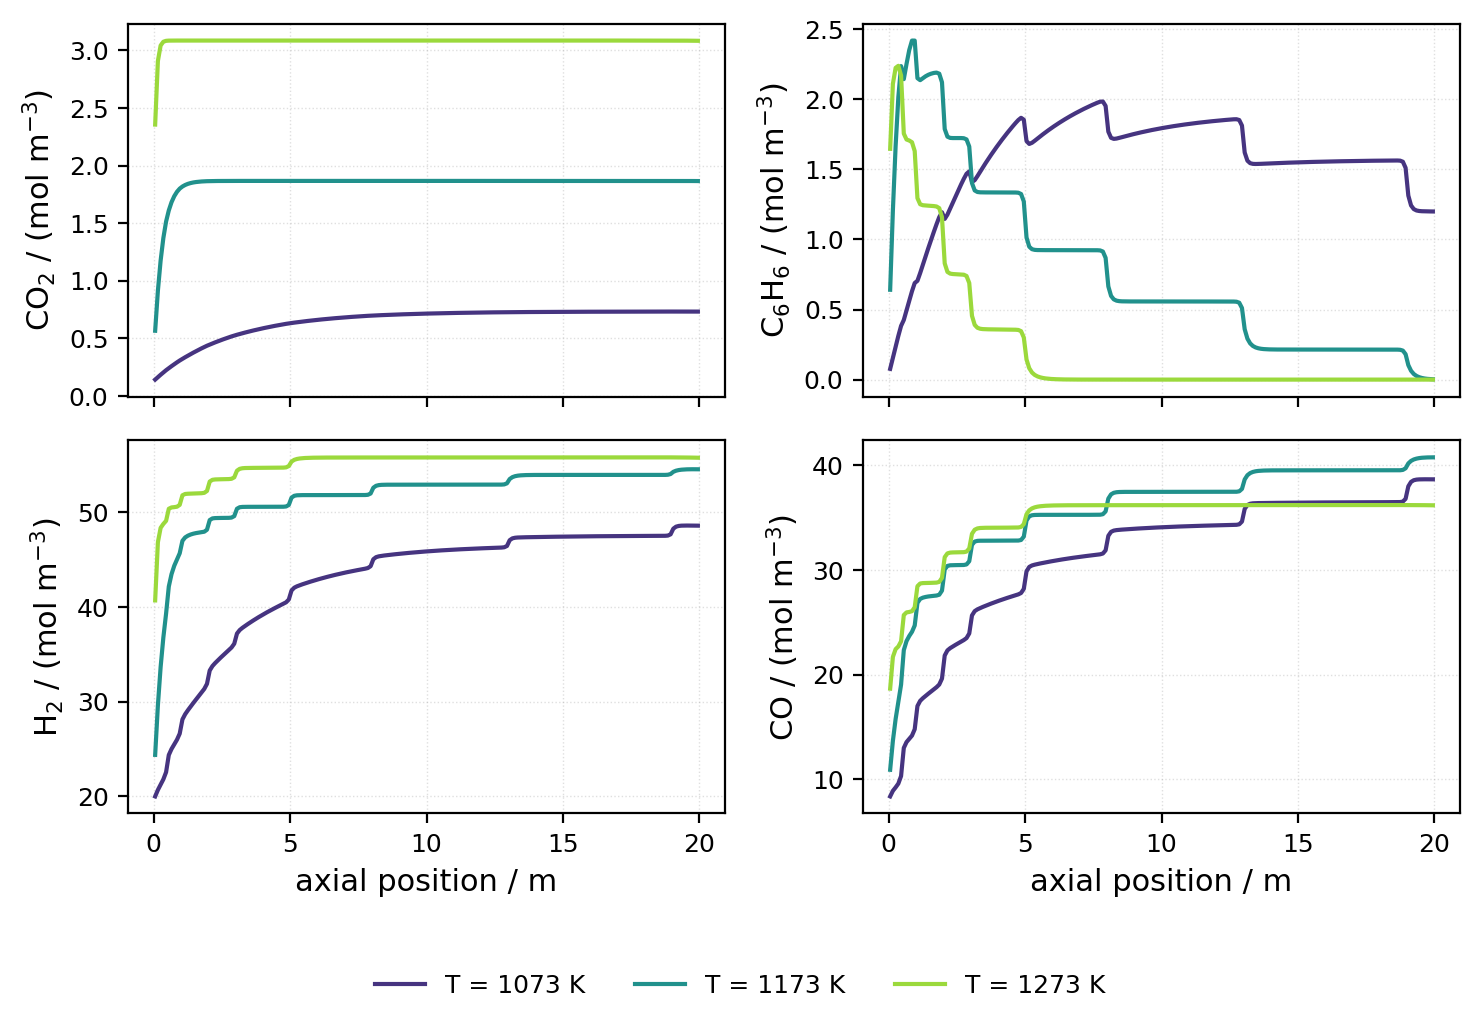
\includegraphics[width=0.95\textwidth]{figures/profiles_T_sweep.png}
\caption{Steady-state profiles of four key species (CO\(_2\), C\(_6\)H\(_6\), H\(_2\), CO) at three reactor temperatures, \(T \in \{1073, 1173, 1273\}\,\si{\kelvin}\), at the design feed velocity \(u = \SI{0.516}{\metre\per\second}\).}\label{fig:profiles_T}
\end{figure}

The first knob is the reactor temperature itself --- the most direct control in any reforming process, since every Arrhenius rate constant in the kinetic scheme depends exponentially on it. \Cref{fig:profiles_T} shows the response of the four indicator species to a \(\pm \SI{100}{\kelvin}\) excursion around the design temperature. The dominant signal is on CO\(_2\), whose outlet concentration rises monotonically from \SI{0.73}{\mole\per\metre\cubed} at \(T = \SI{1073}{\kelvin}\) through \SI{1.87}{\mole\per\metre\cubed} at the design point to \SI{3.08}{\mole\per\metre\cubed} at \(T = \SI{1273}{\kelvin}\) --- a four-fold span set by the temperature sensitivity of the \(\alpha\)-methylstyrene steam-reforming reaction (R6), which is the model's sole CO\(_2\) source. R6 has the highest activation energy of the steam-reforming family, and its rate accelerates by roughly an order of magnitude across the \SI{200}{\kelvin} range, driving the CO\(_2\) yield up in proportion. 

The temperature lever also resolves the residual-tar question: at \(T = \SI{1073}{\kelvin}\) the benzene steam-reforming reaction (R5) is too slow to consume C\(_6\)H\(_6\) within the available residence time, and a non-trivial \SI{1.2}{\mole\per\metre\cubed} of benzene arrives at the outlet --- a tar-slip regime; at \(T = \SI{1173}{\kelvin}\) consumption is essentially complete by \(x \approx \SI{15}{\metre}\); at \(T = \SI{1273}{\kelvin}\) the tar is gone within the first few metres.

The H\(_2\) outlet shows a saturating response (\(\SI{48.6}{} \to \SI{54.6}{} \to \SI{55.8}{\mole\per\metre\cubed}\)) and the CO outlet is non-monotonic (\(\SI{38.7}{} \to \SI{40.8}{} \to \SI{36.1}{\mole\per\metre\cubed}\)). The dip at the highest temperature traces back to a temperature-driven shift in the dominant \(\alpha\)-methylstyrene consumption pathway. Integrated reaction-rate diagnostics from the same runs show R3 (partial oxidation, 9 CO and no CO\(_2\) per mole of C\(_9\)H\(_{10}\)) falling from \SI{31}{\percent} of the aromatic-conversion flux at \(T = \SI{1073}{\kelvin}\) to \SI{3}{\percent} at \(T = \SI{1273}{\kelvin}\), while R6 (steam reforming, 6.5 CO and 2.5 CO\(_2\) per mole) rises from \SI{5}{\percent} to \SI{31}{\percent} over the same range. The two channels effectively swap positions; because R6 carries a CO\(_2\) coefficient that R3 lacks, the swap diverts approximately 2.5 mol of carbon per converted \(\alpha\)-methylstyrene from CO into CO\(_2\), and the CO outlet falls despite the total aromatic-conversion rate remaining unchanged. The H\(_2\)/CO ratio at the outlet shifts correspondingly from \(\approx 1.26\) at \SI{1073}{\kelvin} to \(\approx 1.54\) at \SI{1273}{\kelvin}.

In engineering terms, the design point sits just above the tar-clearance threshold: a setpoint excursion downward by \SI{100}{\kelvin} would push the reactor into a tar-slip regime, while an upward excursion of the same magnitude yields a marginally more hydrogen-rich syngas at the cost of accelerated soot formation, with the soot peak growing from \(\SI{3e-4}{\mole\per\metre\cubed}\) at \SI{1073}{\kelvin} through \(\SI{0.007}{\mole\per\metre\cubed}\) at the design point to \(\SI{0.06}{\mole\per\metre\cubed}\) at \SI{1273}{\kelvin} --- a two-orders-of-magnitude excursion across the \SI{200}{\kelvin} range.

\subsection{Feed-velocity variation}\label{ssec:profiles_u}

\begin{figure}[H]
\centering
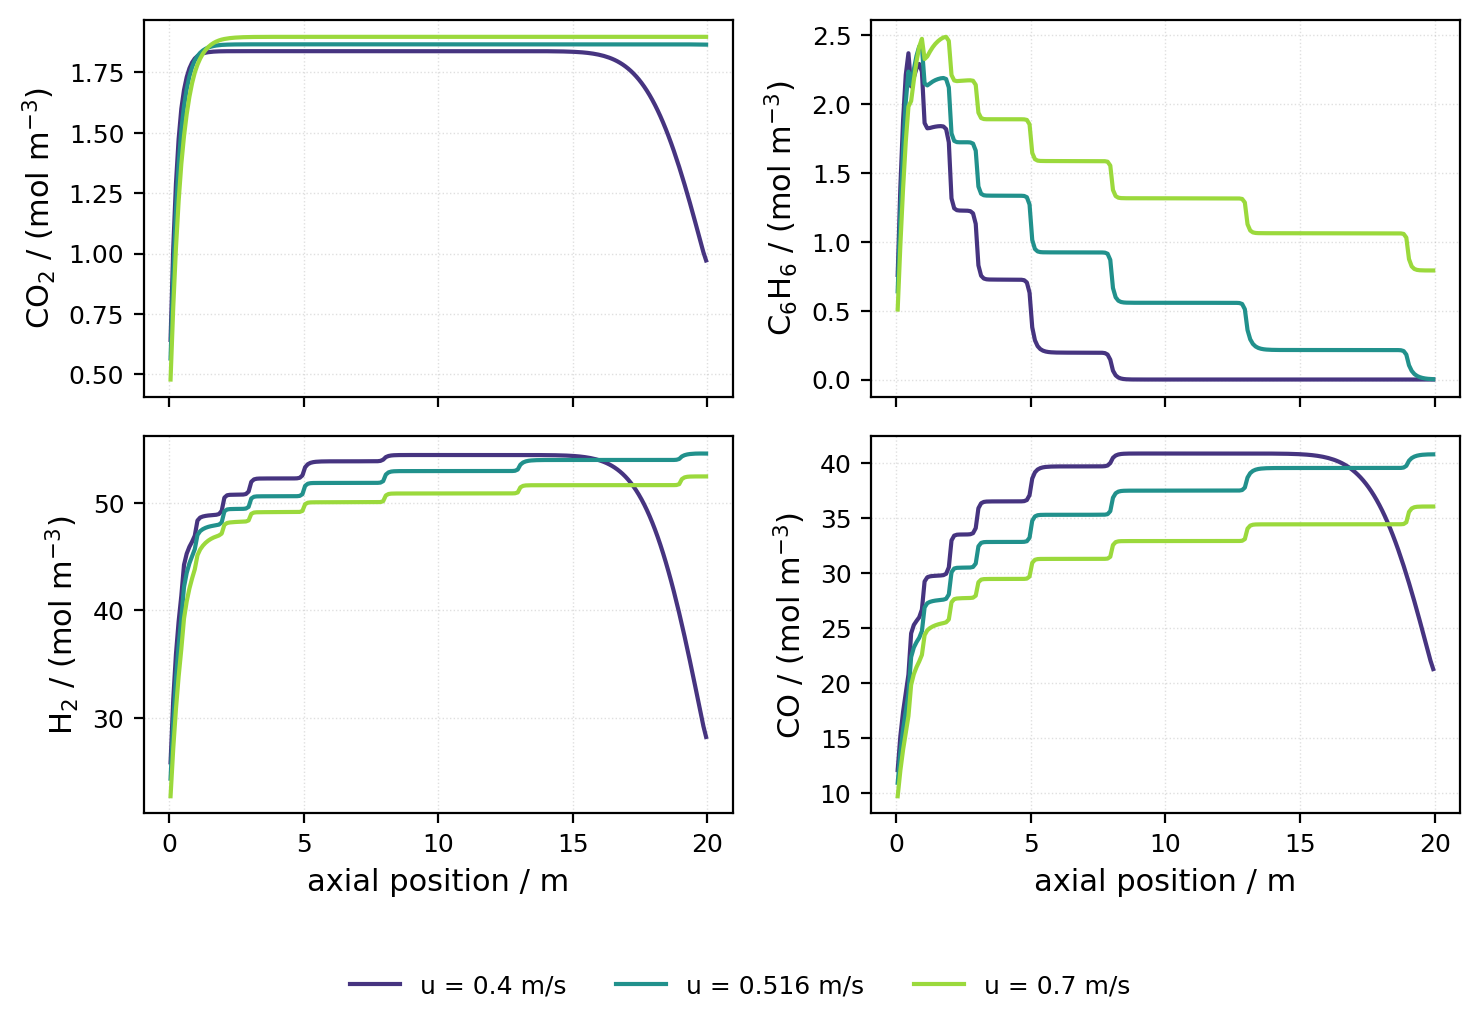
\includegraphics[width=0.95\textwidth]{figures/profiles_u_sweep.png}
\caption{Steady-state profiles of four key species (CO\(_2\), C\(_6\)H\(_6\), H\(_2\), CO) at three feed velocities, \(u \in \{0.400, 0.516, 0.700\}\,\si{\metre\per\second}\) (77~\%, 100~\%, and 136~\% of the design feed velocity, respectively), at the design temperature \(T = \SI{1173.15}{\kelvin}\).}\label{fig:profiles_u}
\end{figure}

The second knob, feed velocity, is harder to move in operation: it is set by the upstream feeder rather than the reactor itself. But moving it on paper reveals what the design value is protecting against. \Cref{fig:profiles_u} shows the response of the four indicator species to a residence-time variation of \(\tau \in \{50, 38.8, 28.6\}\,\si{\second}\), set by the inlet velocity. The clearest engineering signal is on the H\(_2\) and CO profiles at the longest residence time (\(u = \SI{0.4}{\metre\per\second}\), purple curve): both species drop sharply between \(x \approx 17\) and \SI{20}{\metre} as the last side injector at \(x = \SI{19}{\metre}\) delivers an O\(_2\) pulse that, at the slow feed velocity, finds enough downstream residence time to over-oxidise the products. 

The H\(_2\) outlet drops from a mid-reactor maximum of \(\approx \SI{55}{\mole\per\metre\cubed}\) to \SI{28.2}{\mole\per\metre\cubed} at the outlet; CO drops from \(\approx \SI{40}{}\) to \SI{21.2}{\mole\per\metre\cubed}. At the design feed velocity (teal curve) the same last-injector pulse is convected past the outlet before its O\(_2\) is exhausted, and the major-species concentrations remain essentially flat through the back half of the reactor. At the highest feed velocity (\(u = \SI{0.7}{\metre\per\second}\), green curve) the residence time is no longer sufficient to complete benzene steam reforming and \SI{0.79}{\mole\per\metre\cubed} of C\(_6\)H\(_6\) arrives at the outlet --- a partial tar-slip. 

\newpage

The feed-velocity lever therefore exhibits two competing failure modes at the extremes: over-oxidation at low feed velocity and under-conversion at high feed velocity. The design value at \(u = \SI{0.516}{\metre\per\second}\) sits in the narrow window between them where neither failure mode is active. Unlike the temperature lever, which is a candidate process knob during operation, the feed velocity is fixed by the upstream feeder and serves more as a sensitivity check on the operating design than as an active control variable. The third lever has neither limitation.

\subsection{Side-injection flow-rate variation}\label{ssec:profiles_F}

\begin{figure}[H]
\centering
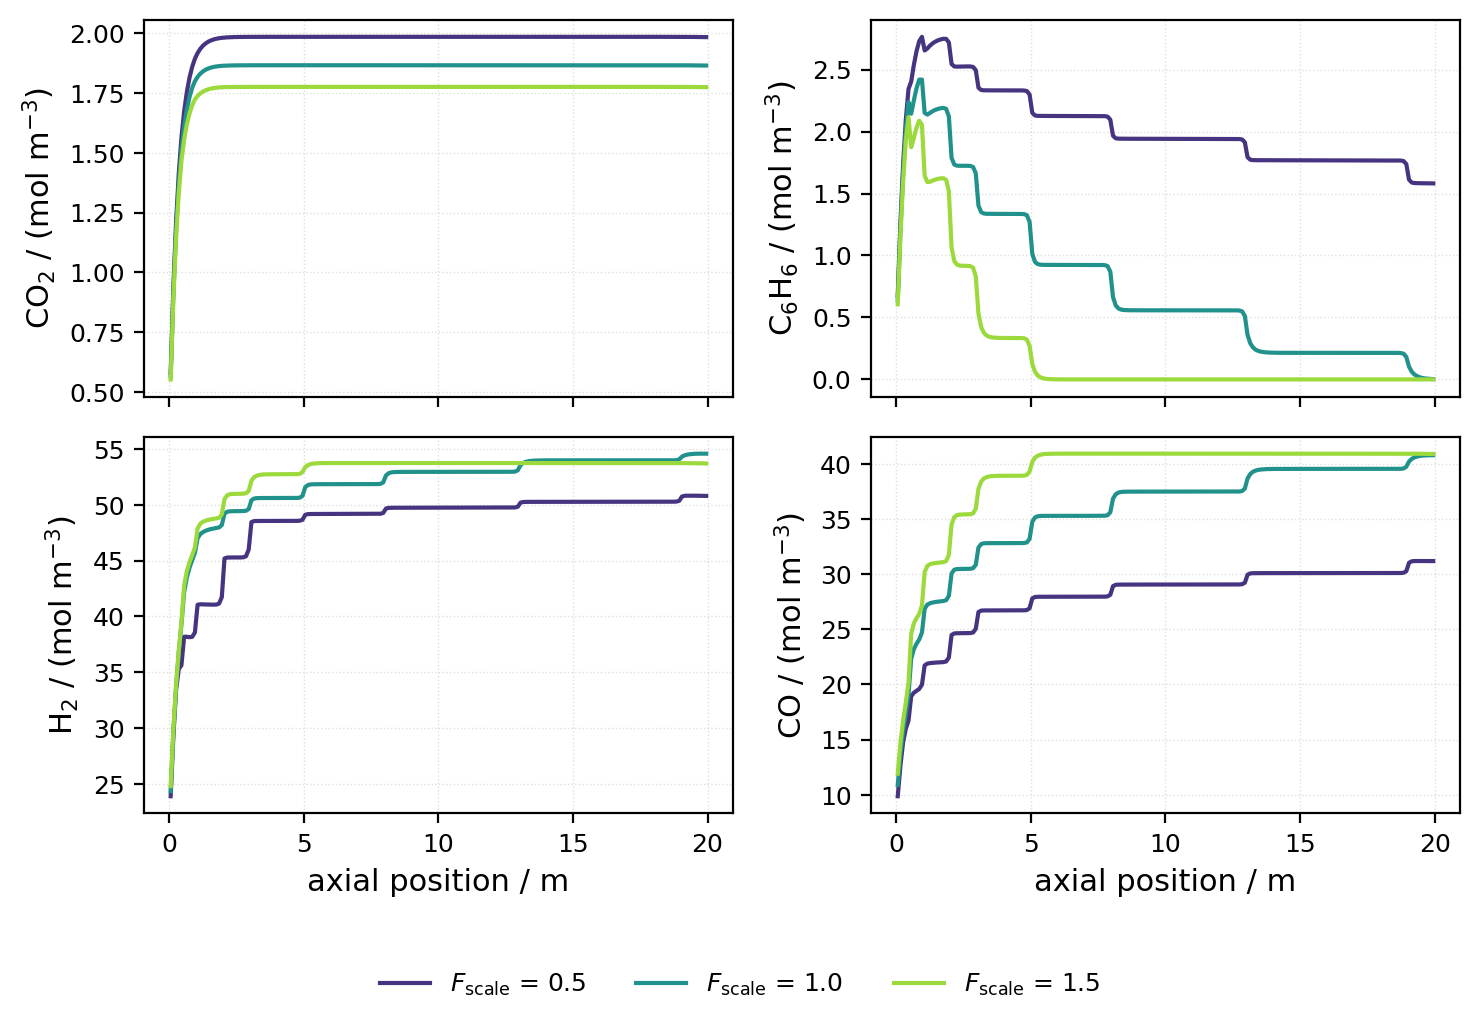
\includegraphics[width=0.95\textwidth]{figures/profiles_F_sweep.png}
\caption{Steady-state profiles of four key species (CO\(_2\), C\(_6\)H\(_6\), H\(_2\), CO) at three values of the side-injection mass-flow multiplier, \(F_\mathrm{scale} \in \{0.5, 1.0, 1.5\}\), at the design temperature and feed velocity. \(F_\mathrm{scale}\) multiplies every active injector uniformly, so the H\(_2\)O/O\(_2\) split ratio is preserved.}\label{fig:profiles_F}
\end{figure}

The third and final knob is the total mass flow delivered by the side-stream injectors. Unlike the feed velocity, it is genuinely under the reactor operator's control --- every injector has its own valve. And unlike the temperature, which lifts every Arrhenius rate uniformly, the side-injection flow probes the chemistry asymmetrically: the same multiplier hits the steam supply (which feeds reforming) and the oxygen supply (which feeds partial oxidation), so the optimum, if there is one, must come from the balance between those two channels. \Cref{fig:profiles_F} shows the response of the four indicator species to a \(\pm 50\,\%\) variation of the global side-injection mass flow. This variation differs from the \(T\) and \(u\) variations in one important respect: it exhibits a non-monotonic optimum within the tested range. 

At \(F_\mathrm{scale} = 0.5\) the under-fed reactor cannot supply enough H\(_2\)O to reform the benzene formed at the inlet, so a residual \SI{1.58}{\mole\per\metre\cubed} of C\(_6\)H\(_6\) persists along the second half of the reactor and arrives at the outlet --- a tar-slip more severe than the \(T = \SI{1073}{\kelvin}\) case; the H\(_2\) and CO outlets are correspondingly depressed (\SI{50.8}{} and \SI{31.2}{\mole\per\metre\cubed} respectively, against \SI{54.6}{} and \SI{40.8}{\mole\per\metre\cubed} at the design value). At \(F_\mathrm{scale} = 1.0\) the benzene is fully reformed by \(x \approx \SI{13}{\metre}\) and the major-species outlets reach the design-case values. At \(F_\mathrm{scale} = 1.5\) the H\(_2\) yield decreases marginally to \SI{53.7}{\mole\per\metre\cubed} while the CO outlet is essentially unchanged. 

The slight H\(_2\) drop reflects two effects of the uniform multiplier: the additional O\(_2\) delivered alongside the additional steam pushes a larger fraction of the hydrocarbon feed through the partial-oxidation channels (R1--R3), which yield fewer H\(_2\) per carbon than the corresponding steam-reforming reactions (R4--R6), and the higher overall injection flow modestly dilutes the outlet stream. Neither outlet is materially shifted, but the additional steam does suppress the soot peak from \SI{0.0066}{} to \SI{0.0026}{\mole\per\metre\cubed} (R5, the model's sole carbon-forming step, slowed relative to R8 gasification by the excess steam). 

The injection-flow rate therefore behaves as a calibration knob with a clear optimum near the design point: under-feeding starves benzene reforming, over-feeding plateaus the syngas yield while consuming additional steam-injector capacity. Of the three variations, this is the only one with a non-monotonic optimum inside the tested range. The design point sits very close to that optimum, which makes the side-injection flow rate the most directly actionable of the three control knobs for any future parametric optimisation of the reactor.

% ===========================================================================
\section{Performance: Wall-Clock vs Grid Resolution}\label{sec:walltime_test}
% ===========================================================================

The performance comparison begins with a wall-clock scaling test. The real eight-reaction isothermal reactor model is integrated from \(t = 0\) to \(t_\mathrm{end} = \SI{50}{\second}\) by each of the three solvers, at six grid resolutions, \(N_{\mathrm{cells}} \in \{50, 100, 200, 400, 800, 1000\}\). Each (solver, grid) combination is a single run; the measurement is the total CPU time reported by the integrator's internal timer, excluding output I/O.

\begin{figure}[H]
\centering
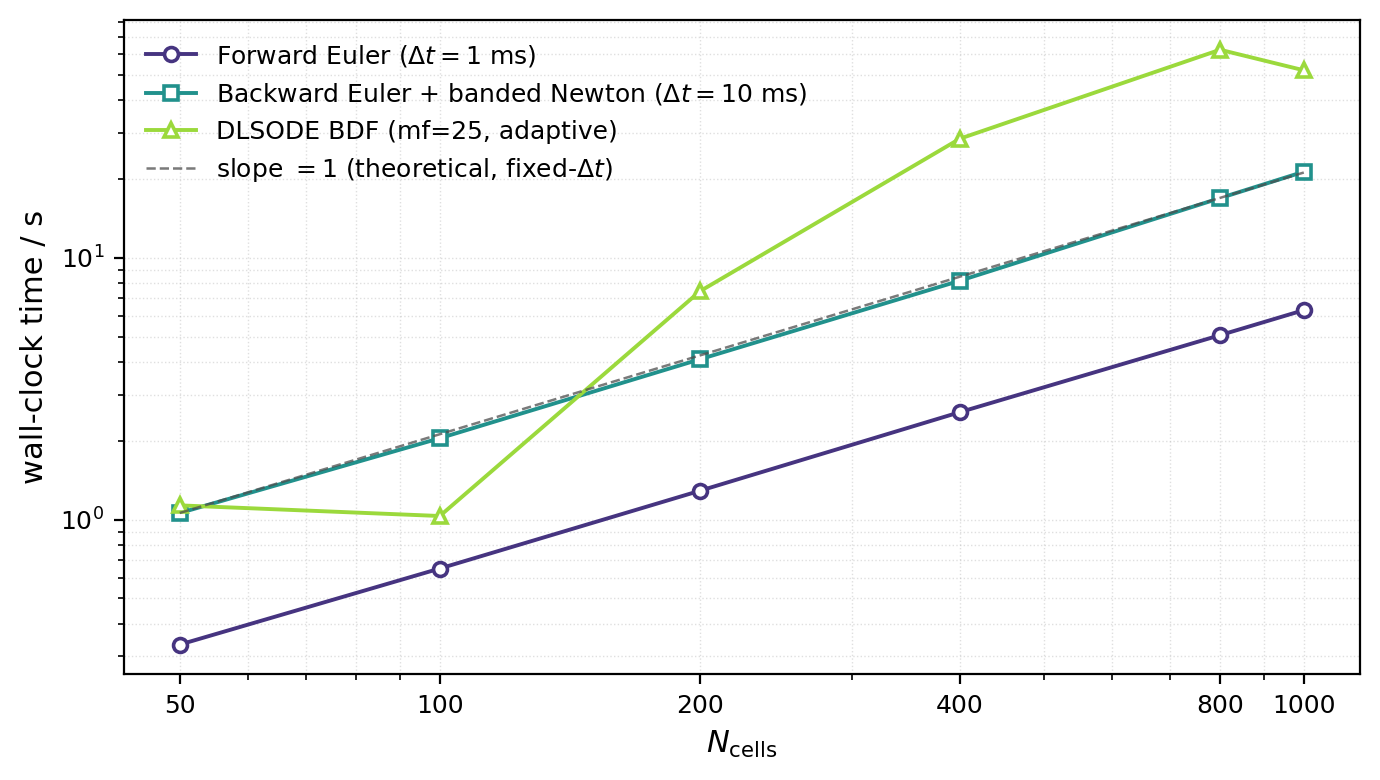
\includegraphics[width=0.95\textwidth]{figures/test1_walltime.png}
\caption{Wall-clock time vs grid resolution on the real eight-reaction isothermal reactor model, integrated to \(t_\mathrm{end} = \SI{50}{\second}\). In log-log coordinates, forward Euler and backward Euler scale linearly with \(N_\mathrm{cells}\) under fixed \(\Delta t\); DLSODE is non-monotonic, reflecting variable BDF order and adaptive step selection.}\label{fig:test1_walltime}
\end{figure}

\Cref{fig:test1_walltime} shows the result. Forward Euler and backward Euler follow the slope-one scaling expected of a fixed-\(\Delta t\) integrator on a banded right-hand side: per-step work scales linearly with \(N_\mathrm{cells}\) (banded Jacobian factorisation for backward Euler; banded RHS evaluation for forward Euler), while the step count \(t_\mathrm{end}/\Delta t\) is grid-independent. Forward Euler is roughly three times faster than backward Euler at every grid, reflecting the absence of a Newton iteration per step. 

The cube-of-\(N\) scaling that an explicit method might exhibit near the diffusive CFL boundary does not surface here: at \(\Delta t = \SI{1}{\milli\second}\) the integrator sits well below the CFL bound (\(\sim\SI{20}{\milli\second}\) at \(N_\mathrm{cells} = 1{,}000\)) throughout the sweep. DLSODE displays a non-monotonic wall-clock profile. The integrator is fastest at \(N_\mathrm{cells} = 100\) (\SI{1.03}{\second}, BDF order four), grows steadily through \(N_\mathrm{cells} = 200\) and \(400\), peaks at \(N_\mathrm{cells} = 800\) at \SI{62.4}{\second} --- slower than at the finer \(N_\mathrm{cells} = 1{,}000\) grid --- and partially recovers to \SI{52.1}{\second} at the finest resolution. 

\newpage

Inspection of the internal counters explains the peak: at \(N_\mathrm{cells} = 800\) the BDF order has collapsed to one and DLSODE has reverted in practice to backward Euler, with the internal step count rising to 22{,}856; at \(N_\mathrm{cells} = 1{,}000\) the integrator escalates BDF back to order five with substantially fewer steps. The pattern is characteristic of variable-order adaptive schemes when the local-truncation-error estimator persistently rejects high-order steps: the scheme remains A-stable but loses its order advantage, and the overhead of the predictor--corrector difference and order-selection logic sits on top of what are effectively backward-Euler numerics. DLSODE's adaptive machinery therefore provides robustness without guaranteeing monotonic performance scaling: on the present model, the integrator outperforms the fixed-step alternatives only near \(N_\mathrm{cells} = 100\) and is otherwise the slowest of the three.

% ===========================================================================
\section{Accuracy: Relative Error vs Grid Resolution}\label{sec:error_test}
% ===========================================================================

The second numerical test anchors the accuracy measurement to a closed-form analytical solution. Because the real eight-reaction model has no such reference, the test uses a simplified plug-flow reactor in which the eight Arrhenius reactions are replaced by a single first-order irreversible step, with all geometry, hydrodynamics, and discretisation choices inherited from the real model. The nine side-stream injectors are switched off for this test, so the simplified reactor receives reactant only through the Dirichlet inlet. The simplification yields a linear convection--diffusion--reaction equation whose steady-state solution is available in closed form, and the simulation--reference gap is then a clean measurement of the spatial-discretisation error of the FVM scheme that is shared by all three solvers.

\subsection{Test problem and analytical solution}\label{ssec:test_problem_analytical}

The reduced model retains the geometry of \cref{tab:reactor_params} (\(L = \SI{20}{\metre}\), \(u = \SI{0.516}{\metre\per\second}\), \(D_\mathrm{ax} = \SI{1e-2}{\metre\squared\per\second}\)), the first-order upwind FVM stencil, and the same three time-integration algorithms. Only the chemistry is replaced: the eight Arrhenius reactions of the real model reduce to a single first-order step
\begin{equation}
  \ce{A -> B}, \qquad r = k\,C_A,
  \label{eq:test2_reaction}
\end{equation}
with \(k = \SI{0.026}{\per\second}\) chosen so that the Damköhler number \(\mathrm{Da} = kL/u \approx 1\) --- the reaction timescale matches the residence time, giving a non-trivial conversion across the reactor. The Péclet number inherited from the geometry, \(\mathrm{Pe} = uL/D_\mathrm{ax} \approx 1{,}032\), places the test problem in the same strongly convection-dominated regime as the real reactor.

The steady-state mass balance for species~A is the linear ODE
\begin{equation}
  \underbrace{D_\mathrm{ax}\,\frac{\mathrm{d}^2 C_A}{\mathrm{d}x^2}}_{\text{diffusion}}
  \;-\;
  \underbrace{u\,\frac{\mathrm{d} C_A}{\mathrm{d}x}}_{\text{convection}}
  \;-\;
  \underbrace{k\,C_A}_{\text{reaction}}
  \;=\; 0,
  \qquad x \in [0, L],
  \label{eq:test2_steady_pde}
\end{equation}
subject to the same boundary conditions the FVM stencil enforces: a Dirichlet inlet \(C_A(0) = C_{A,\mathrm{in}}\) and a zero-gradient (Neumann) outlet \(\mathrm{d}C_A/\mathrm{d}x(L) = 0\). The derivation that follows is the standard reactor-engineering treatment of convection--diffusion--reaction systems, presented in detail by Levenspiel~\cite{Levenspiel1999} and Fogler~\cite{Fogler2006}. Non-dimensionalising with \(x^\ast = x/L\) and substituting the trial solution \(C_A \propto e^{\lambda\,x^\ast}\) yields the characteristic equation \(\lambda^2 - \mathrm{Pe}\,\lambda - \mathrm{Pe}\,\mathrm{Da} = 0\), whose two roots are
\begin{equation*}
  \lambda_\pm \;=\; \frac{\mathrm{Pe}}{2}\left(1 \pm \beta\right),
  \qquad
  \beta \;=\; \sqrt{1 + 4\,\mathrm{Da}/\mathrm{Pe}}.
\end{equation*}
Here \(\beta\) is the bookkeeping symbol that comes out of the quadratic equation. With our parameters (\(\mathrm{Pe} = 1{,}032\), \(\mathrm{Da} \approx 1\)) the value \(\beta = \sqrt{1 + 4/1032} \approx 1.002\) is barely above unity, and the two eigenvalues evaluate to \(\lambda_+ \approx 1{,}033\) and \(\lambda_- \approx -1\). The general solution \(C_A(x^\ast) = A\,e^{\lambda_+\,x^\ast} + B\,e^{\lambda_-\,x^\ast}\) is therefore the sum of a violently growing exponential and a gently decaying one. The growing branch reaches \(e^{1033}\) at the reactor outlet --- a number with no physical meaning in any concentration --- so its coefficient \(A\) must be of order \(e^{-1033}\), numerically zero for any practical purpose. The Neumann outlet condition pins \(A\) at exactly that level, well below the FVM discretisation errors that the test is designed to measure. Dropping the growing branch and applying the Dirichlet inlet \(C_A(0) = C_{A,\mathrm{in}}\) leaves a single decaying exponential,
\begin{equation}
  \frac{C_A(x^\ast)}{C_{A,\mathrm{in}}} \;=\; e^{\lambda_-\,x^\ast}
  \;\simeq\; \exp(-\mathrm{Da}\,x^\ast),
  \label{eq:test2_analytical}
\end{equation}
where the second equality follows from the Taylor expansion \(\beta = 1 + 2\,\mathrm{Da}/\mathrm{Pe} + \mathcal{O}(1/\mathrm{Pe}^2)\), giving \(\lambda_- = (\mathrm{Pe}/2)(1 - \beta) \simeq -\mathrm{Da}\) to leading order in \(1/\mathrm{Pe}\), and recovers the textbook plug-flow conversion law for a first-order reaction --- a useful sanity check, since at very high Péclet the dispersion term is negligible and the reactor should behave as pure plug flow. At \(\mathrm{Da} \approx 1\) this corresponds to an overall conversion of \(1 - e^{-1} \approx 63\%\). The species~B concentration follows from mass conservation, \(C_B(x^\ast) = C_{A,\mathrm{in}} - C_A(x^\ast)\). \Cref{eq:test2_analytical} is the analytical reference against which the second test measures simulation error.

The boundary conditions of the analytical reference deserve a brief note. The canonical analytical solution for steady-state convection--diffusion--reaction in a tubular reactor assumes Danckwerts (closed--closed) boundaries and is reproduced in standard reactor-engineering textbooks~\cite{Levenspiel1999}. The first-order upwind FVM does not enforce Danckwerts inlet but a simpler Dirichlet ghost cell, so a comparison against the closed--closed reference would conflate spatial-discretisation error with a constant boundary-condition mismatch of order \(1/\mathrm{Pe}\). \Cref{eq:test2_analytical} matches the boundary conditions the FVM actually applies and is therefore the cleaner reference for measuring spatial-discretisation error in isolation.

\subsection{Results}\label{ssec:test2_results}

The error metric reported below is the steady-state max-norm relative error,
\begin{equation}
  \varepsilon_\infty \;=\; \frac{\lVert C_A^{\mathrm{num}} - C_A^{\mathrm{ref}}\rVert_\infty}{\lVert C_A^{\mathrm{ref}}\rVert_\infty},
  \label{eq:max_norm_relerr}
\end{equation}
where the maximum is taken over all \(N_\mathrm{cells}\) FVM cells and the analytical reference \(C_A^{\mathrm{ref}}(x)\) of \cref{eq:test2_analytical} is independent of \(N_\mathrm{cells}\); the figure plots how the numerical solution converges to this fixed reference under grid refinement.

\begin{figure}[!ht]
\centering
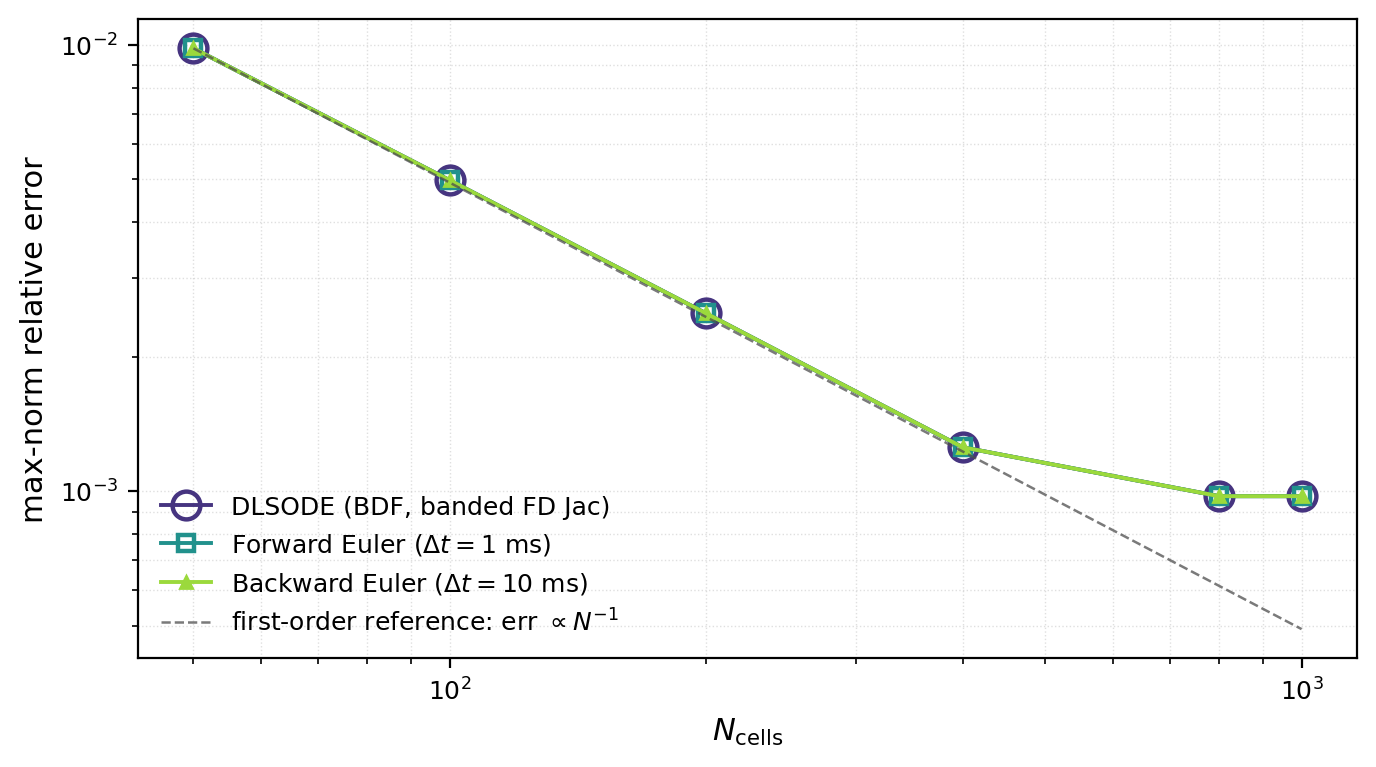
\includegraphics[width=0.95\textwidth]{figures/test2_error_vs_ncells.png}
\caption{Steady-state max-norm relative error of the simulated \(C_A\) profile against the analytical reference of \cref{eq:test2_analytical}, at six grid resolutions. The three solvers' data points overlap to four significant figures at every grid; the dashed line is the slope-(\(-1\)) reference for first-order upwind FVM.}\label{fig:test2_error}
\end{figure}

\Cref{fig:test2_error} shows the result --- and the surprise. The three solvers' data points overlap to four significant figures at every grid. Forward Euler, backward Euler, and DLSODE are accuracy-equivalent on this test at every \(N_\mathrm{cells}\) tested; the time-integration error sits below the spatial-discretisation floor for every solver, at every grid. The error trend tracks the slope-(\(-1\)) reference line closely from \(N_\mathrm{cells} = 50\) (\SI{9.82e-3}{}) to \(N_\mathrm{cells} = 400\) (\SI{1.25e-3}{}), the convergence rate predicted for the first-order upwind convection scheme. From \(N_\mathrm{cells} = 800\) onward the error plateaus at approximately \SI{9.75e-4}{}, consistent with the absolute tolerance \(\mathrm{atol} = 10^{-9}\) of the reference DLSODE run propagating into the rel-err denominator and the residual incomplete steady-state convergence at the integration window \(t_\mathrm{end} = \SI{200}{\second}\) used for this test. The overlap of the three solvers is itself the key result. On a linear test problem, the implicit Newton iteration of backward Euler converges in a single step --- the residual is exact at any \(\Delta t\) --- and the variable-order BDF formulae of DLSODE reduce in practice to backward Euler at order one; in both cases the time integration is free of truncation error to within the rounding floor, leaving only the FVM upwind scheme to set the accuracy. This is the spatial-discretisation floor: the best accuracy any of the three solvers can achieve at a given grid, regardless of how cheaply or expensively that accuracy is reached.

% ===========================================================================
\section{Explicit vs Implicit Euler Crossover}\label{sec:euler_comparison}
% ===========================================================================

The two tests above benchmark each solver at its default configuration. They do not, however, answer a more practical question: at what time step does the implicit method's per-step Newton overhead become cheaper than the explicit method's tighter step bound? This section probes that crossover. Backward Euler is run at five time steps, \(\Delta t \in \{5, 10, 25, 50, 100\}\,\si{\milli\second}\), against an explicit-Euler reference at its CFL-bounded \(\Delta t = \SI{1}{\milli\second}\). All six configurations are swept over the same four grid resolutions, \(N_\mathrm{cells} \in \{100, 200, 400, 800\}\), giving 24 runs in total.

\begin{figure}[H]
\centering
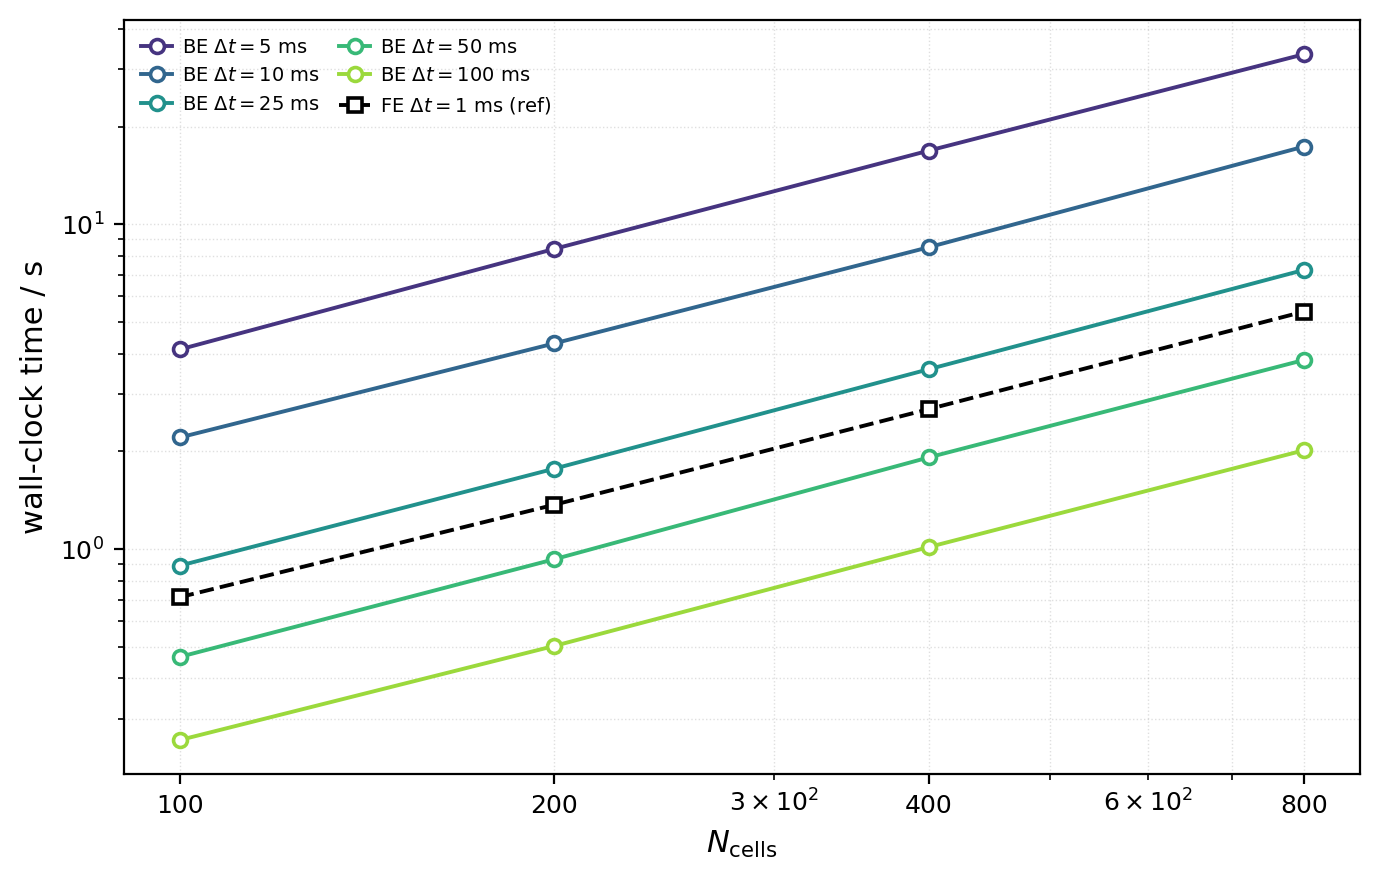
\includegraphics[width=0.95\textwidth]{figures/cpu_vs_n.png}
\caption{Wall-clock time vs grid resolution for forward Euler at \(\Delta t = \SI{1}{\milli\second}\) (dashed reference) and backward Euler at five time steps \(\Delta t \in \{5, 10, 25, 50, 100\}\,\si{\milli\second}\) (solid lines, viridis palette). All solvers integrate the real eight-reaction model from \(t = 0\) to \(t_\mathrm{end} = \SI{50}{\second}\).}\label{fig:cpu_vs_n}
\end{figure}

\Cref{fig:cpu_vs_n} shows the result. The structure of the comparison is itself unsurprising: all six curves --- the forward-Euler reference (dashed) and the five backward-Euler sweeps at increasing \(\Delta t\) (solid, viridis) --- follow the same slope-one scaling in log-log coordinates, because the per-step work of the banded Newton iteration scales linearly with \(\mathrm{NEQ} = N_\mathrm{cells}\cdot N_s\), and the total wall-clock time is therefore proportional to \(N_\mathrm{cells}\) at any fixed \(\Delta t\). The vertical spacing between the backward-Euler curves is set by the time-step ratio: doubling \(\Delta t\) approximately halves the wall time, since the typical Newton iteration count per step is essentially independent of \(\Delta t\) (\(\approx 25\) RHS evaluations per step at every grid in the sweep). What the comparison resolves is where backward Euler crosses the forward-Euler reference.

The forward-Euler reference falls between the backward-Euler curves at \(\Delta t = \SI{25}{\milli\second}\) and \(\Delta t = \SI{50}{\milli\second}\). At \(N_\mathrm{cells} = 400\), for instance, forward Euler at \(\Delta t = \SI{1}{\milli\second}\) takes \SI{2.7}{\second}, against \SI{3.6}{\second} for backward Euler at \(\Delta t = \SI{25}{\milli\second}\) and \SI{1.9}{\second} at \(\Delta t = \SI{50}{\milli\second}\). The crossover lies near \(\Delta t \approx \SI{25}{\milli\second}\) on this model and is independent of \(N_\mathrm{cells}\) across the tested range --- the two scaling laws are parallel, so the relative ordering of the integrators does not depend on grid resolution. The decisive moment of the test is at the largest backward-Euler step tested. At \(\Delta t = \SI{100}{\milli\second}\), backward Euler advances the real model to \(t_\mathrm{end} = \SI{50}{\second}\) in \SI{2.0}{\second} at \(N_\mathrm{cells} = 800\) against \SI{5.4}{\second} for forward Euler at the same grid --- a 2.7-fold acceleration that takes backward Euler from the slowest fixed-step integrator at its default settings (\cref{fig:test1_walltime}) to the fastest of the three at a tuned step.
% ===========================================================================
\section{Discussion and Solver Recommendation}\label{sec:ch4_discussion}
% ===========================================================================

The three numerical tests above converge on a single solver recommendation for the present model. \Cref{fig:test2_error} establishes that all three solvers reach the same spatial-discretisation floor at every grid: forward Euler, backward Euler, and DLSODE are accuracy-equivalent at any target \(N_\mathrm{cells}\) on the linear test problem. \Cref{fig:test1_walltime} then ranks them by cost on the real eight-reaction stiff model: forward Euler is the fastest of the three at every grid in the sweep, with backward Euler approximately a factor of three slower and DLSODE either marginally competitive at \(N_\mathrm{cells} = 100\) or, at higher resolutions, materially penalised by the BDF-order-collapse pathology described above. For a target relative error of \(\sim 10^{-3}\) (corresponding to \(N_\mathrm{cells} \approx 400\) in the error plot), forward Euler integrates the real model in \SI{2.6}{\second}, against \SI{8.2}{\second} for backward Euler and \SI{28.6}{\second} for DLSODE. The recommendation is therefore forward Euler at the default \(\Delta t = \SI{1}{\milli\second}\) --- the cheapest of the three integrators at the established accuracy floor. This recommendation comes with two important caveats.

\newpage

The first concerns the scope of the accuracy ranking, which is established on the linear simplified PFR and cannot be transposed verbatim to the stiff Arrhenius chemistry of the real model, where the time-integration error of forward Euler at \(\Delta t = \SI{1}{\milli\second}\) might no longer be below the spatial floor. A direct measurement of the time-integration error on the real model would require an analytical reference for the eight-reaction system, which does not exist; the indirect ranking provided by the second test is therefore the strongest accuracy claim available within the scope of this work. Within that limitation, the empirical result is unambiguous: at the engineering-relevant grids around \(N_\mathrm{cells} \approx 400\), forward Euler at the default \(\Delta t = \SI{1}{\milli\second}\) agrees with the DLSODE reference to within the spatial-discretisation floor of \cref{fig:test2_error}, and at materially lower wall-clock-time cost. 

The recommendation comes at a cost: the user must keep \(\Delta t\) within the conditional stability bound of forward Euler --- a discipline that adaptive methods like DLSODE assume on the user's behalf, and that backward Euler dispenses with through unconditional A-stability. \Cref{fig:cpu_vs_n} sharpens the picture further: when the user is willing to find a large stable time step for backward Euler --- here, \(\Delta t = \SI{100}{\milli\second}\) is stable and converges Newton at every grid tested --- backward Euler is the fastest of the three integrators on this model, displacing forward Euler from the top of the wall-clock ranking. The default-configuration ranking and the tuned ranking therefore disagree, and the choice between them is a deployment decision rather than a numerical one.

The second caveat looks forward rather than back. The recommendation rests on the present kinetic scheme and on the isothermal assumption --- eight Arrhenius reactions at a fixed operating temperature, which together leave the chemistry-induced stiffness within reach of forward Euler at \(\Delta t = \SI{1}{\milli\second}\). Two model extensions, both realistic next steps from the present work, would push the comparison the other way. The first is a more detailed reaction mechanism --- more species, a wider spread of activation energies, the chemistry one would adopt to model pyrolytic gas faithfully. The second is to relax the isothermal assumption and couple an energy balance to the species equations, so that the temperature, and through the Arrhenius dependence the rate constants, become part of the state vector --- a regime where local temperature excursions can amplify rate constants by orders of magnitude across a single integration step. Either extension would grow the stiffness of the right-hand side and tighten forward Euler's conditional-stability bound on \(\Delta t\).

\newpage

In the limit where the chemical timescale falls below the present transport-dominated bound, forward Euler will either choke or be forced into impractically small steps, and the constant per-step overhead of an implicit method becomes economical by comparison. DLSODE is built for exactly this regime: adaptive BDF order and predictor--corrector step-size control absorb the stiffness without user intervention, and the wall-clock-time penalty seen in \cref{fig:test1_walltime} on the present model would then be the price paid for robustness on a problem where the explicit scheme is no longer admissible. For either model extension the comparison would need to be re-run; based on what we see here, the ranking is likely to flip, with DLSODE moving ahead of forward Euler. On the present model, however, the answer is forward Euler.

% ===========================================================================
% chapters/conclusions.tex — Conclusions
% ===========================================================================

\chapter*{Conclusions}
\addcontentsline{toc}{chapter}{Conclusions}
\markboth{CONCLUSIONS}{CONCLUSIONS}

This thesis has developed and exercised a dynamic mathematical model of a non-catalytic tubular reformer for pyrolytic gas, and has benchmarked three time-integration algorithms on the resulting stiff convection--diffusion--reaction system. The work delivers three artefacts: a ten-species, eight-reaction lumped kinetic scheme calibrated for iso-thermal operation; a one-dimensional plug-flow reactor with staged side-stream injection, discretised by first-order upwind finite volumes; and an integrator recommendation that meets the spatial-discretisation accuracy floor at materially lower cost than the alternatives.

The engineering results show a reactor with a narrow but real design margin. The temperature lever exposes a tar-clearance threshold just below the design point: at \(T = \SI{1073}{\kelvin}\) benzene steam reforming is too slow to consume the aromatic load within the available residence time, and a non-trivial tar-slip arrives at the outlet. The feed-velocity lever reveals two competing failure modes at the extremes --- over-oxidation at low feed velocity and under-conversion at high --- with the design value sitting in the narrow window between them. The side-injection flow-rate variation is the only one of the three with a non-monotonic optimum inside the tested range, and the design point sits close to that optimum. It is therefore the most directly actionable knob for any future parametric optimisation.

The numerical results identify forward Euler at \(\Delta t = \SI{1}{\milli\second}\) as the cheapest integrator that meets the accuracy floor at the engineering-relevant grid. Backward Euler at a tuned \(\Delta t = \SI{100}{\milli\second}\) is faster still, at the cost of user-side stability tuning; DLSODE provides default-configuration robustness but is penalised on the present iso-thermal model by a BDF-order-collapse pathology at fine grids. The recommendation is therefore tied to the present kinetic scheme and operating point: a richer reaction mechanism or a coupled energy balance would tighten the explicit method's stability bound and shift the ranking toward the implicit alternatives. Both extensions are natural directions for follow-on work, and the parametric studies in this thesis define the operating range over which the resulting model should be tested.


% =============================================================================
% BACK MATTER — Bibliography
% =============================================================================
\newpage
\singlespacing%
\footnotesize
\bibliographystyle{unsrt}
\bibliography{references/references}

% --- List of Symbols + List of Abbreviations ---
\normalsize
\singlespacing%
% ===========================================================================
% chapters/symbols_and_abbreviations.tex — List of Symbols + List of Abbreviations
% ===========================================================================

\chapter*{List of Symbols}
\addcontentsline{toc}{chapter}{List of Symbols}
\markboth{LIST OF SYMBOLS}{LIST OF SYMBOLS}

\begin{longtable}{@{} p{0.16\textwidth} p{0.60\textwidth} p{0.18\textwidth} @{}}
\(A\)                   & cross-sectional area                                              & \si{\square\metre}                                  \\
\(C_i\)                 & molar concentration of species \(i\)                              & \si{\mole\per\cubic\metre}                          \\
\(C_{i,\mathrm{in}}\)   & inlet concentration of species \(i\)                              & \si{\mole\per\cubic\metre}                          \\
\(C_{\mathrm{tot}}\)    & total molar concentration                                         & \si{\mole\per\cubic\metre}                          \\
\(d\)                   & tube internal diameter                                            & \si{\metre}                                         \\
\(D_{AB}\)              & molecular diffusivity of species A in B                           & \si{\square\metre\per\second}                       \\
\(D_{\mathrm{ax}}\)     & axial dispersion coefficient                                      & \si{\square\metre\per\second}                       \\
\(D_{\mathrm{num}}\)    & numerical (artificial) diffusion coefficient                      & \si{\square\metre\per\second}                       \\
\(\mathrm{Da}\)         & Damk\"ohler number                                                & ---                                                 \\
\(E_i\)                 & activation energy of reaction \(i\)                               & \si{\kilo\joule\per\mole}                           \\
\(E(t)\)                & residence-time distribution function                              & \si{\per\second}                                    \\
\(F^{\mathrm{c}}\)      & convective molar flux at a cell face                              & \si{\mole\per\square\metre\per\second}              \\
\(F^{\mathrm{d}}\)      & diffusive molar flux at a cell face                               & \si{\mole\per\square\metre\per\second}              \\
\(F_{\mathrm{scale}}\)  & global side-injection mass-flow multiplier                        & ---                                                 \\
\(\mathbf{f}\)          & right-hand-side vector of the semi-discrete ODE system            & \si{\mole\per\cubic\metre\per\second}               \\
\(\mathbf{g}\)          & Newton residual vector                                            & \si{\mole\per\cubic\metre}                          \\
\(\mathbf{J}\)          & Jacobian matrix                                                   & varies                                              \\
\(k_i(T)\)              & temperature-dependent rate constant of reaction \(i\)             & varies                                              \\
\(L\)                   & reactor length                                                    & \si{\metre}                                         \\
\(\mathrm{mf}\)         & DLSODE method flag                                                & ---                                                 \\
\(\mathrm{ML}\)         & lower half-bandwidth of the Jacobian                              & ---                                                 \\
\(\mathrm{MU}\)         & upper half-bandwidth of the Jacobian                              & ---                                                 \\
\(N_{\mathrm{cells}}\)  & number of finite-volume cells                                     & ---                                                 \\
\(N_{\mathrm{eqs}}\)    & total number of ODE equations                                     & ---                                                 \\
\(N_s\)                 & number of species                                                 & ---                                                 \\
\(P\)                   & total pressure                                                    & \si{\pascal}                                        \\
\(\mathrm{Pe}\)         & P\'eclet number                                                   & ---                                                 \\
\(\mathrm{Pe}_{\mathrm{cell}}\) & cell P\'eclet number                                      & ---                                                 \\
\(\mathrm{Pe}_d\)       & Bodenstein number                                                 & ---                                                 \\
\(r_i\)                 & net volumetric production rate of species \(i\)                   & \si{\mole\per\cubic\metre\per\second}               \\
\(R\)                   & universal gas constant                                            & \si{\joule\per\mole\per\kelvin}                     \\
\(\mathrm{Re}\)         & Reynolds number                                                   & ---                                                 \\
\(\mathrm{rtol}\)       & relative tolerance of the adaptive integrator                     & ---                                                 \\
\(\mathrm{atol}\)       & absolute tolerance of the adaptive integrator                     & ---                                                 \\
\(S_{i,j}\)             & side-injection source term for species \(i\) in cell \(j\)        & \si{\mole\per\cubic\metre\per\second}               \\
\(T\)                   & reactor temperature                                               & \si{\kelvin}                                        \\
\(t\)                   & time                                                              & \si{\second}                                        \\
\(t_{\mathrm{end}}\)    & integration time horizon                                          & \si{\second}                                        \\
\(u\)                   & inlet feed velocity                                               & \si{\metre\per\second}                              \\
\(V\)                   & cell volume                                                       & \si{\cubic\metre}                                   \\
\(x\)                   & axial coordinate                                                  & \si{\metre}                                         \\
\(\mathbf{y}\)          & state vector of all species concentrations                        & \si{\mole\per\cubic\metre}                          \\
\(y_{i,\mathrm{in}}\)   & inlet mole fraction of species \(i\)                              & ---                                                 \\
\(\beta\)               & characteristic-root intermediate variable                         & ---                                                 \\
\(\Delta t\)            & time step                                                         & \si{\second}                                        \\
\(\Delta x\)            & finite-volume cell width                                          & \si{\metre}                                         \\
\(\lambda_\pm\)         & characteristic equation eigenvalues                               & ---                                                 \\
\(\nu\)                 & kinematic viscosity                                               & \si{\square\metre\per\second}                       \\
\(\rho_{\mathrm{soot}}\)& soot mass concentration                                           & \si{\kilo\gram\per\cubic\metre}                     \\
\(\sigma\)              & Taylor smearing distance                                          & \si{\metre}                                         \\
\(\tau\)                & mean residence time                                               & \si{\second}                                        \\
\end{longtable}

\chapter*{List of Abbreviations}
\addcontentsline{toc}{chapter}{List of Abbreviations}
\markboth{LIST OF ABBREVIATIONS}{LIST OF ABBREVIATIONS}

\begin{longtable}{@{} p{0.16\textwidth} p{0.78\textwidth} @{}}
AI       & artificial intelligence                                                 \\
BDF      & backward differentiation formula                                        \\
CFL      & Courant--Friedrichs--Lewy (number / stability condition)                \\
CSTR     & continuous stirred-tank reactor                                         \\
FVM      & finite-volume method                                                    \\
GRI-Mech & Gas Research Institute methane mechanism                                \\
ODE      & ordinary differential equation                                          \\
ODEPACK  & Hindmarsh's package of ODE solvers                                      \\
PAH      & polycyclic aromatic hydrocarbon                                         \\
PDE      & partial differential equation                                           \\
PFR      & plug-flow reactor                                                       \\
RTD      & residence-time distribution                                             \\
\end{longtable}


\end{document}
